%%%%%%%%%%%%%%%%%%%%%%%%%%%%%%%%%%%%%%%%%%%%%%%%%%%%%%%%%%%%%%%
%%%  Glassines in one dimensional hopping model
%%%%%%%%%%%%%%%%%%%%%%%%%%%%%%%%%%%%%%%%%%%%%%%%%%%%%%%%%%%%%%%

\documentclass[aps,pre,floats,floatfix,fleqn,notitlepage]{revtex4-1}
%\documentclass[twocolumns,fleqn,aps,pra,floats,floatfix]{revtex4}
%\documentclass[aps,pra,floats,floatfix]{revtex4-1}
%\documentclass[aps,pra,floats,floatfix,twocolumn]{revtex4}

\def \thebibliography#1{
\noindent {\bf References:}
\list
{\relax}{
\setlength{\labelsep}{2mm}
\setlength{\itemindent}{0mm}
\setlength{\leftmargin}{6mm}
\setlength{\itemsep}{-0.3mm}
}
\def\newblock{\hskip .11em plus .33em minus .07em}
\sloppy\clubpenalty4000\widowpenalty4000\sfcode`\.=1000\relax}

% special 
\usepackage{ifthen}
\usepackage{ifpdf}
\usepackage{color}
%
%\ifpdf
%\usepackage{graphicx}
%\usepackage{epstopdf}
%\else
\usepackage{graphicx}
\usepackage{epsfig}
%\fi
\graphicspath{{/Users/danielhurowitz/PROJ/NHR/Figs/}{/Users/danielhurowitz/PROJ/NEG/Figs/}{./}}

% fonts
\usepackage{latexsym}
\usepackage{amsmath}
\usepackage{amssymb}
\usepackage{bm}
\usepackage{wasysym}

%\usepackage{hyperref}

%%%%%%%%%%%%%%%%%%%%%%%%%%%%%%%%%%%%%%%%%%%%%%%%%%%%%%%%%%%%%%%%

% NEW 
\newcommand{\abs}[1]{\left|#1\right|}
\newcommand{\Prob}{\mbox{Prob}\,}
\newcommand{\erf}{\mbox{erf}\,}

% math symbols I
\newcommand{\sinc}{\mbox{sinc}}
\newcommand{\const}{\mbox{const}}
\newcommand{\trc}{\mbox{trace}}
\newcommand{\intt}{\int\!\!\!\!\int }
\newcommand{\ointt}{\int\!\!\!\!\int\!\!\!\!\!\circ\ }
\newcommand{\ar}{\mathsf r}
\newcommand{\im}{\mbox{Im}}
\newcommand{\re}{\mbox{Re}}

% math symbols II
\newcommand{\eexp}{\mbox{e}^}
\newcommand{\bra}{\left\langle}
\newcommand{\ket}{\right\rangle}

% Mass symbol
\newcommand{\mass}{\mathsf{m}} 
\newcommand{\Mass}{\mathsf{M}} 

% more math commands
\newcommand{\tbox}[1]{\mbox{\tiny #1}}
\newcommand{\bmsf}[1]{\bm{\mathsf{#1}}} 
%\newcommand{\amatrix}[1]{\matrix{#1}} 
\newcommand{\amatrix}[1]{\begin{matrix} #1 \end{matrix}} 
\newcommand{\pd}[2]{\frac{\partial #1}{\partial #2}}

% equations
%\newcommand{\mylabel}[1] {\textcolor{blue}{[#1]}\label{#1}} %{\label{#1}}
\newcommand{\mylabel}[1]{\label{#1}}  %{\textcolor{blue}{[#1]}\label{#1}}

%\newcommand{\mylabel}[1] {} %{\label{#1}}
\newcommand{\beq}{\begin{eqnarray}}
\newcommand{\eeq}{\end{eqnarray}} 
\newcommand{\be}[1]{\begin{eqnarray}\ifthenelse{#1=-1}{\nonumber}{\ifthenelse{#1=0}{}{\mylabel{e#1}}}}
\newcommand{\ee}{\end{eqnarray}} 

% arrangement
\newcommand{\drawline}{\begin{picture}(500,1)\line(1,0){500}\end{picture}}
\newcommand{\bitem}{$\bullet$ \ \ \ }
\newcommand{\Cn}[1]{\begin{center} #1 \end{center}}
\newcommand{\mpg}[2][1.0\hsize]{\begin{minipage}[b]{#1}{#2}\end{minipage}}
\newcommand{\mpgt}[2][1.0\hsize]{\begin{minipage}[t]{#1}{#2}\end{minipage}}
\newcommand{\putgraph}[2][width=0.30\hsize]{\includegraphics[#1]{#2}}

% more
\newcommand{\Eq}[1]{\textcolor{blue}{equation~(\ref{#1})}} %{equation~(\ref{#1})}
\newcommand{\Fig}[1] {\textcolor{blue}{Fig.~\ref{#1}}} %{Fig.~\ref{#1}}
\newcommand{\hide}[1]{\textcolor{red}{[hidden text]}} %{}
\newcommand{\rmrk}[1]{\textcolor{red}{#1}}
%\newcommand{\Rmrk}[1]{\textcolor{blue}{\LARGE\bf #1}}


%\renewcommand{\includegraphics}[2][]{}
\renewcommand{\cite}[1]{\textcolor{blue}{[\onlinecite{#1}}]} %{[\onlinecite{#1}]} 


\def\circbul{{\bigcirc \mkern-8mu _{\bullet} \mkern-8mu}} 


\newcommand{\ola}{\protect\overleftarrow}
\newcommand{\ora}{\protect\overrightarrow}
%%%%%%%%%%%%%%%%%%%%%%%%%%%%%%%%%%%%%%%%%%%%%%%%%%%%%%%%%%%%%%%%%%%%%%%%%%%%%%%%%%%%%%%%%%
%%%%%%%%%%%%%%%%%%%%%%%%%%%%%%%%%%%%%%%%%%%%%%%%%%%%%%%%%%%%%%%%%%%%%%%%%%%%%%%%%%%%%%%%%%
 
\begin{document}

\title{One dimensional hopping model - interplay of resistor-network and Sinai spreading}

\author{Notes by Daniel Hurowitz}

\affiliation{
Department of Physics, Ben-Gurion University of the Negev, P.O.B. 653, Beer-Sheva 84105, Israel
}
\maketitle
%%%%%%%%%%%%%%%%%%%%%%%%%
The conventional view of variable-range-hopping is based on the assumption 
that the rates of transitions are {\em symmetric} 
but have log-wide distribution as in glassy systems. 
Namely, the rate at the $n$th bond is written as 
%
\beq 
g_n \ \ = \ \ \text{rate of transition} \ \ = \ \ \exp(-\mathcal{B}_n)
\eeq
% 
where the barriers $\mathcal{B}_n$ have (say) a box distribution.
Consequently a resistor-network analysis is most appropriate for the 
analysis,leading to an Ohmic result for the current, namely $I\propto 1/L$,  
where $L$ is the length of the sample, but the prefactor is exponentially small. 

Contrary to that Sinai has considered a model where the rates are {\em asymmetric}. 
The asymmetry of transitions in the $n$th bond is characterized by   
%
\beq
\mathcal{E}_n \ \ = \ \ \ln\left( \frac{\ora{w}_{n}}{\ola{w}_{n}} \right)  
\eeq
%  
which we call ``stochastic field". 
At equilibrium $\mathcal{E}_n = (E_{n}-E_{n+1})/T$, 
where $T$ is the temperature.  
More generally we can define a stochastic potential 
%
\beq
V_n \ \ = \ \ \sum_{n'=0}^n \mathcal{E}_{n'}
\eeq
% 
In non-equilibrium circumstances the telescopic correlations are likely 
to be broken, the sum becomes of order $\sqrt{L}$,   
and therefore $I\propto \exp(-\sqrt{L})$ due to this buildup 
of an activation barrier. 
    

%%%%%%%%%%%%%%%%%%%%%%%%%
\section{The model, and main observations}

Below we consider a 1D model were we have an interplay of resistor-network physics 
(due to random couplings) and Sinai physics (due to random stochastic field).       
Specifically we consider an $N$ site ring with near-neighbor transitions.
Each bond is characterized by two numbers:
%
\be{1}
\mathcal{B}_n \ \ &=& \ \ \text{barriers} \ \ = \ \ \text{random} \in [-\Delta,\Delta] \\
\mathcal{E}_n \ \ &=& \ \ \text{stochastic field} \ \ = \ \ \text{random} \in [s-\sigma,s+\sigma] 
\ee
%
Accordingly the transition rates across the $n^{th}$ bond are 
%
\be{1}
\ora{w}_{n} &=&  w_{n+1,n} \ = \ g_n \eexp{ \mathcal{E}_n/2} \ = \ \eexp{-\mathcal{B}_n + \mathcal{E}_n/2} \\
\ola{w}_{n} &=&  w_{n,n+1} \ = \ g_n \eexp{-\mathcal{E}_n/2} \ = \ \eexp{-\mathcal{B}_n - \mathcal{E}_n/2}
\ee
%
The average stochastic field~$s$ is called in the literature ``affinity". 
It can be written as $s=\text{Force}/T$, where the force 
is defined as the slope of the potential, and $T$ is the temperature.
The term ``slope" is appropriate if we view our model as describing 
a periodic lattice with $N$-site unit cell. But we prefer to have in 
mind a ring geometry so the more appropriate notion is ``stochastic motive force":
%
\beq
S_{\circlearrowleft} \ \ = \ \ \sum_{n\in\text{ring}}^N \mathcal{E}_{n} \ \ = \ \ Ns
\eeq  
%
We calculate the drift velocity $v$ and the diffusion coefficient $D$ as a function of the affinity~$s$. 
In the absence of disorder ($\Delta=\sigma=0$) they are related by a {\em generalized} Einstein relations:
%
\beq
\frac{v}{D} \ \ = \ \ \frac{2}{a}\tanh\left(\frac{as}{2}\right)
\eeq
%
where $a=1$ is the lattice constant. 
The traditional Einstein relation $v/D=s$ holds if $s$ is sufficiently small. 
This is usually rephrased as $\text{mobility}/\text{diffusion} = 1/T$.  
The other extreme limit of very large $s$ implies 
unidirectional transitions with $v/D=2/a$. 
The latter ratio reflects Poisson statistics.   
      
Taking the disorder into account the Poisson limit becomes  $v/D=2/a_{\infty}$, 
where $a_{\infty}$ depends on the disorder:
%
%
\be{4}
a_{\infty} \ \ = \ \  \left(\frac{2D}{v}\right)_{s\rightarrow\infty} \ = \ 
\left[\frac{\big\langle (1/\ora{w})^2 \big\rangle}{\big\langle (1/\ora{w}) \big\rangle^2}\right]
\ \  = \  \ \frac{\sigma \Delta}{4} \coth\left( \frac{\sigma}{2} \right)\coth\left( \frac{\Delta}{2} \right)
\ee
%
If we increase $s$ from zero to infinity the ratio $v/D$ has 
a crossover from $v/D=s$ to $v/D=2/a_{\infty}$, which is illustrated in \Fig{fig2}.
Due to the disorder $\sigma$ we get what we call a ``Sinai step". 
This means that for small $s$ the transport is suppressed due to 
the buildup of a potential barrier, while large enough $s$ flattens 
the barrier leading to ``sliding" with large drift velocity.


%%%%%%%%%%%%%%%%%%%%%%%%%%%%%%%%%%%%
\begin{figure}[h]
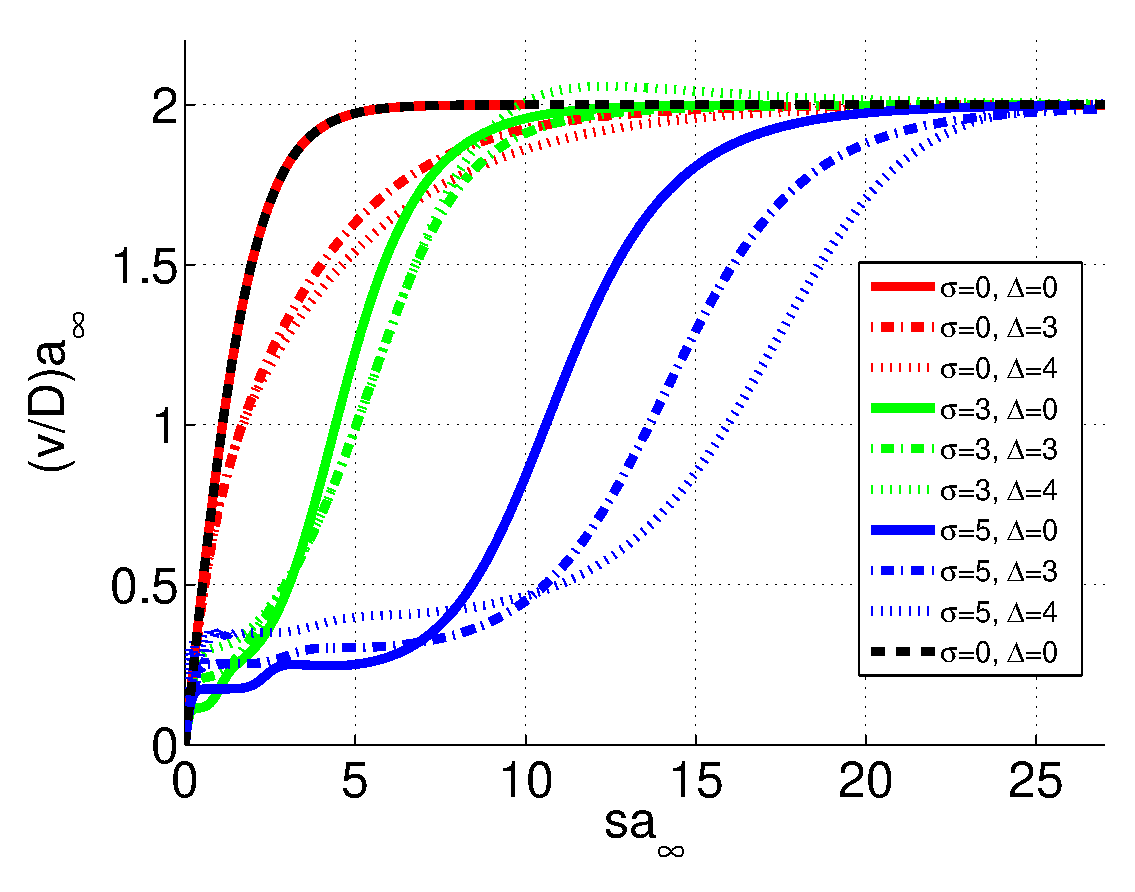
\includegraphics[height=7cm]{/Figs/vD.eps}

\caption{The scaled $v/D$ ratio versus the scaled $s$ for various values of $\sigma$ and $\Delta$.
Different colors correspond to different $\sigma$,  
while different line styles correspond to different $\Delta$. 
The dashed black line $2\tanh(x)$ describes the result 
that would be obtained for a non-disordered model. The number of sites is $N=30$. 
}
\label{fig2}
\end{figure}
%%%%%%%%%%%%%%%%%%%%%%%%%%%%%%%%%%%%%


The additional aspect that we want to analyze is the implication 
of having log-wide distribution of couplings, i.e. having finite $\Delta$.
We observe in  \Fig{fig2} that by increasing $\Delta$ 
the Sinai step is somewhat smeared: the crossover from 
activated transport to sliding becomes wider.

In order to get the "big picture" we calculate the ratio between the scaled $v/D$ 
and the reference curve $2\tanh(x)$ and displays the results as images in \Fig{fig3a}.  
The small $s$ results imply that $\Delta$ has little effect on the 
beginning of the Sinai step. Namely it hardly affects the crossover 
from the linear-response (Einstein) regime to the activated transport (Sinai) regime. 
But the effect of $\Delta$ becomes qualitativley similar 
to the effect of $\sigma$ as we cross from activated transport to "sliding".  


%%%%%%%%%%%%%%%%%%%%%%%%%%%%%%%%%%%%%%%%%%%%%%%%%%%%%%%%%%%%
\begin{figure}[h]

\includegraphics[height=4cm]{/Figs/vD_vDinf_1.eps}
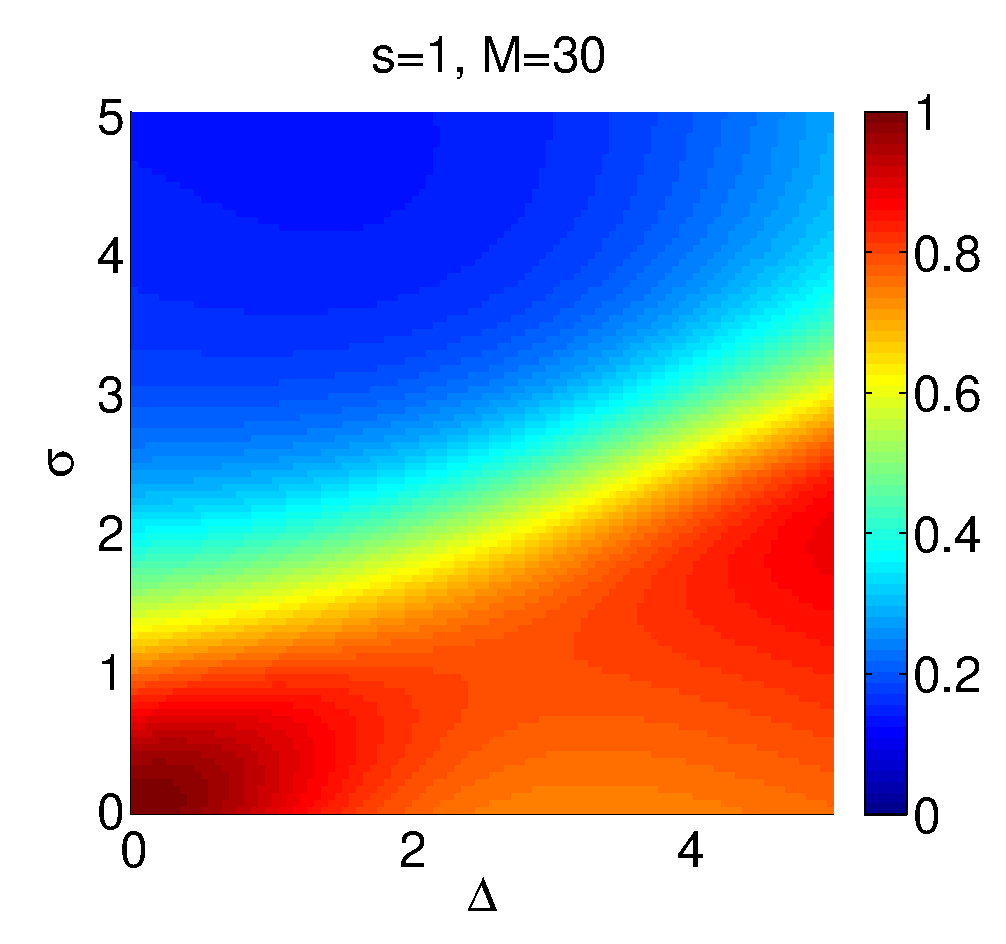
\includegraphics[height=4cm]{/Figs/vD_vDinf_2.eps}
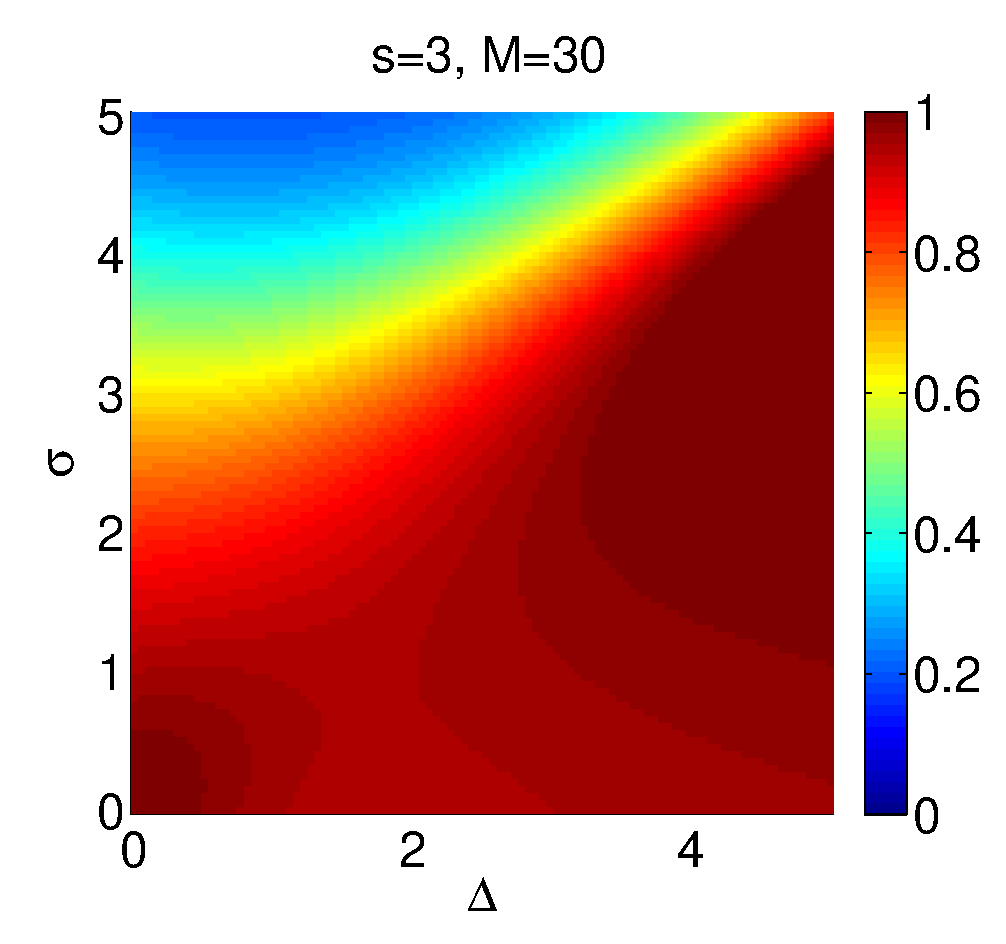
\includegraphics[height=4cm]{/Figs/vD_vDinf_3.eps}
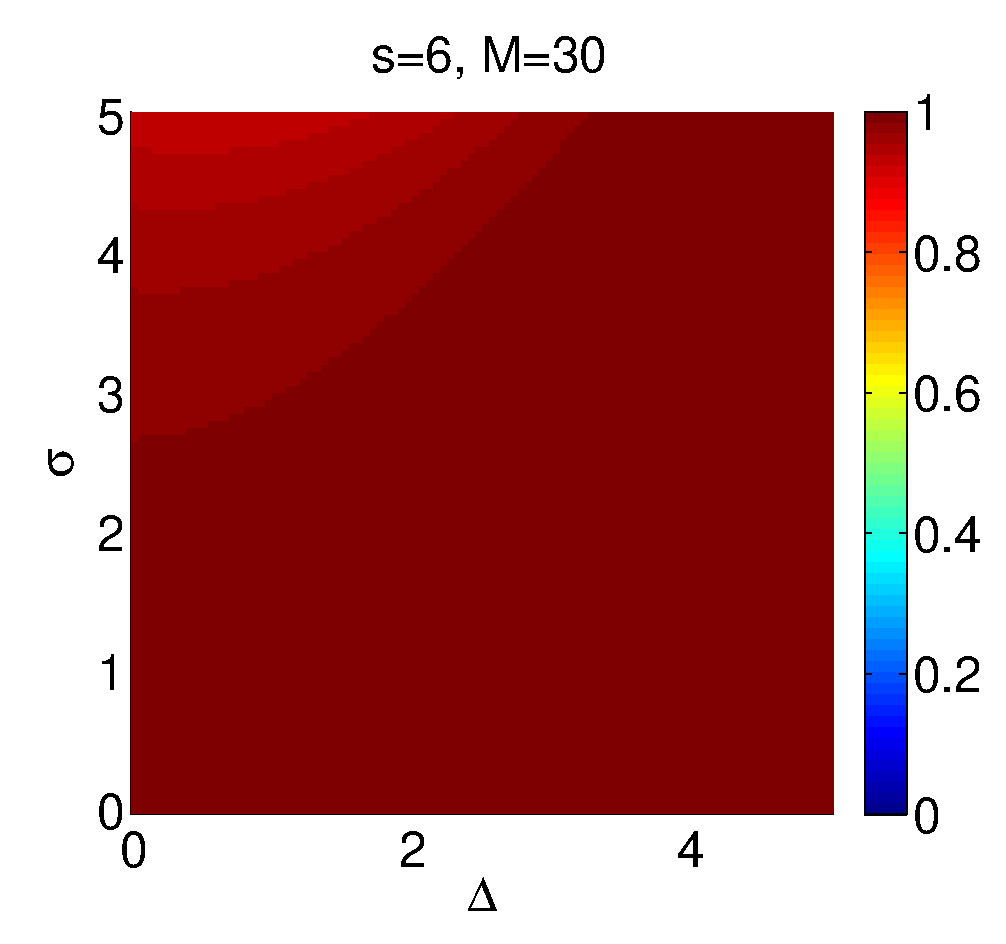
\includegraphics[height=4cm]{/Figs/vD_vDinf_4.eps}

\caption{
The ratio between $a_{\infty} v/D$ and $2\tanh(x)$ is imaged 
as a function of $\Delta$ and $\sigma$ for representative 
values of the affinity (${s=0.1,1,3,6}$). The number of sites is $N=30$.}
\label{fig3a}
\end{figure}


%%%%%%%%%%%%%%%%%%%%%%%%%
\section{A more detailed analysis}

To determine the roles played by $\sigma$ and $\Delta$, we study 
the probability distribution of the displacement $x$.   
In the ring context it is defined as the winding number times~$N$.  
We look at the cumulant generating function
%
\be{3}
g(\lambda) \ \ = \ \ \lim_{t\to \infty} \left[-\frac{1}{t} \ln  \langle \eexp{-\lambda x} \rangle_t \right]
\ee
%
which completely determines the probability distribution in the long time limit. 
Note that $g(\lambda)$ satisfies the non equilibrium fluctuation theorem (NFT) 
%
\beq
g(\lambda) \ = \ g(s -\lambda)
\eeq
%
If the distribution is Gaussian, then $g(\lambda)$ is a parabola
%
\beq
g(\lambda) \ = \ v \lambda -D\lambda^2
\eeq
%
and the NFT implies $v/D=s$. 
This parabola has a maximum at $\lambda=(1/2)v/D$ with height 
%
\beq
h \ \ = \ \ \text{max}[g(\lambda)] \ \ = \ \ \frac{v^2}{4D} \ \ = \frac{1}{4}vs
\eeq
%
Accordingly we use the following dimensionless parameters 
in order to characterize the deviation from Gaussian statistics:
%
\beq
\frac{v/D}{s} \ \ \text{and} \ \ 4\frac{h/v}{s} \ \ \ \ \ \text{[both equal unity for Gaussian statistics]}
\eeq
%
In \Fig{fig3} these two parameters are imaged as a function of $\Delta$ and $\sigma$ 
for representative values of $s$.  For small values of $s$, the ratio $v/Ds$ 
is quite independent of $\Delta$, while as $s$ increases, the effect of $\Delta$ becomes more significant. 


\ \\ \ \\ 

%%%%%%%%%%%%%%%%%%%%%%%%%%%%%%%%%%%%%%%%%%%%
\begin{figure}[h]

\includegraphics[height=4cm]{/Figs/vDs_1.eps}
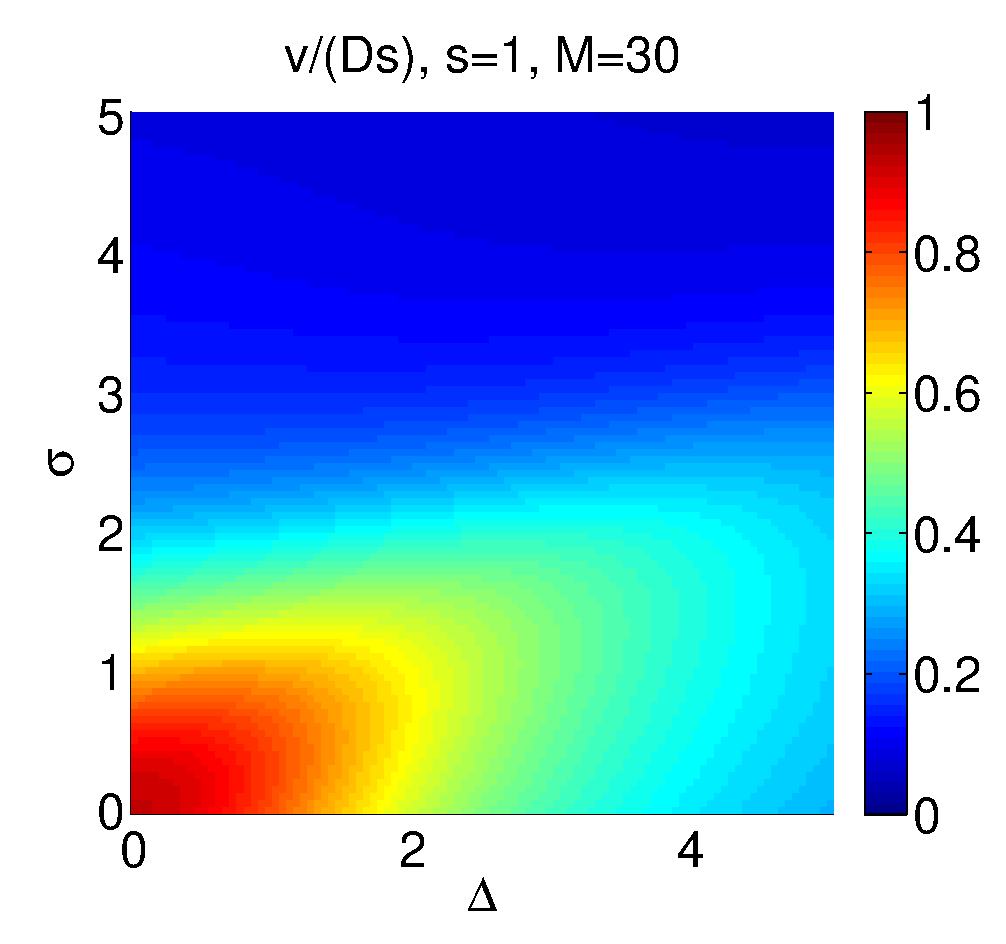
\includegraphics[height=4cm]{/Figs/vDs_2.eps}
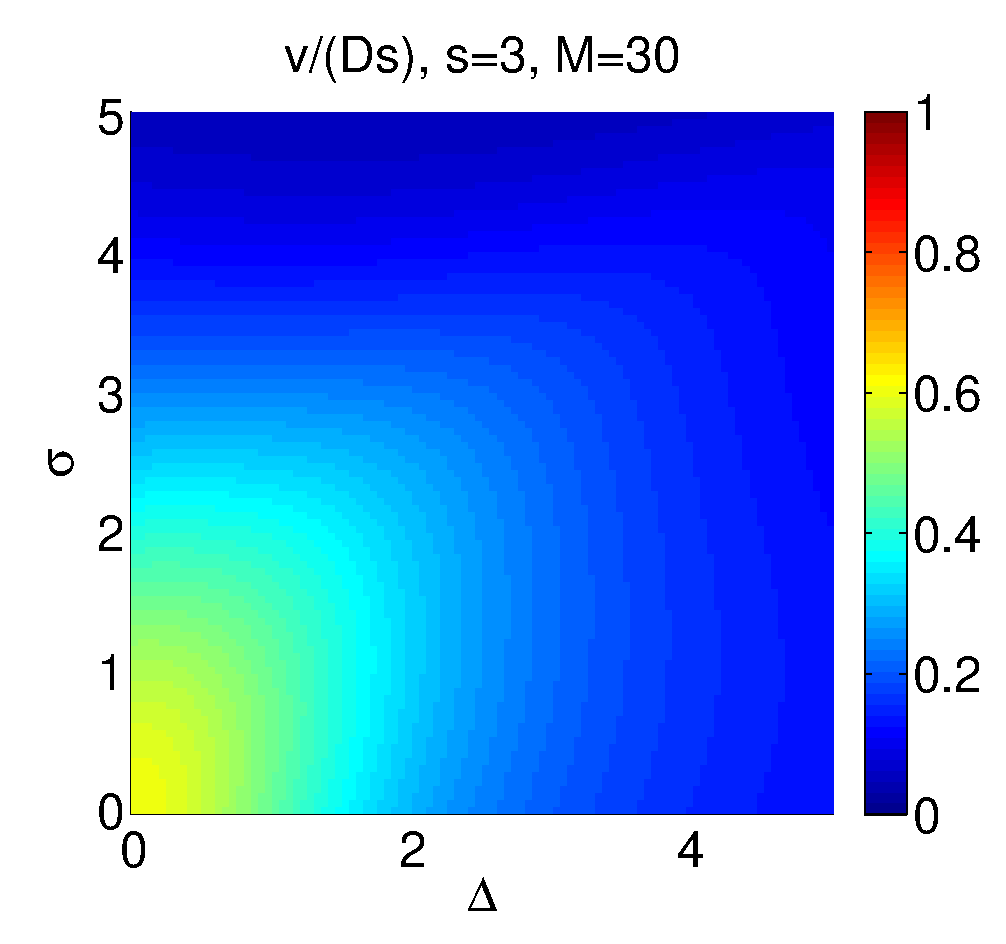
\includegraphics[height=4cm]{/Figs/vDs_3.eps}
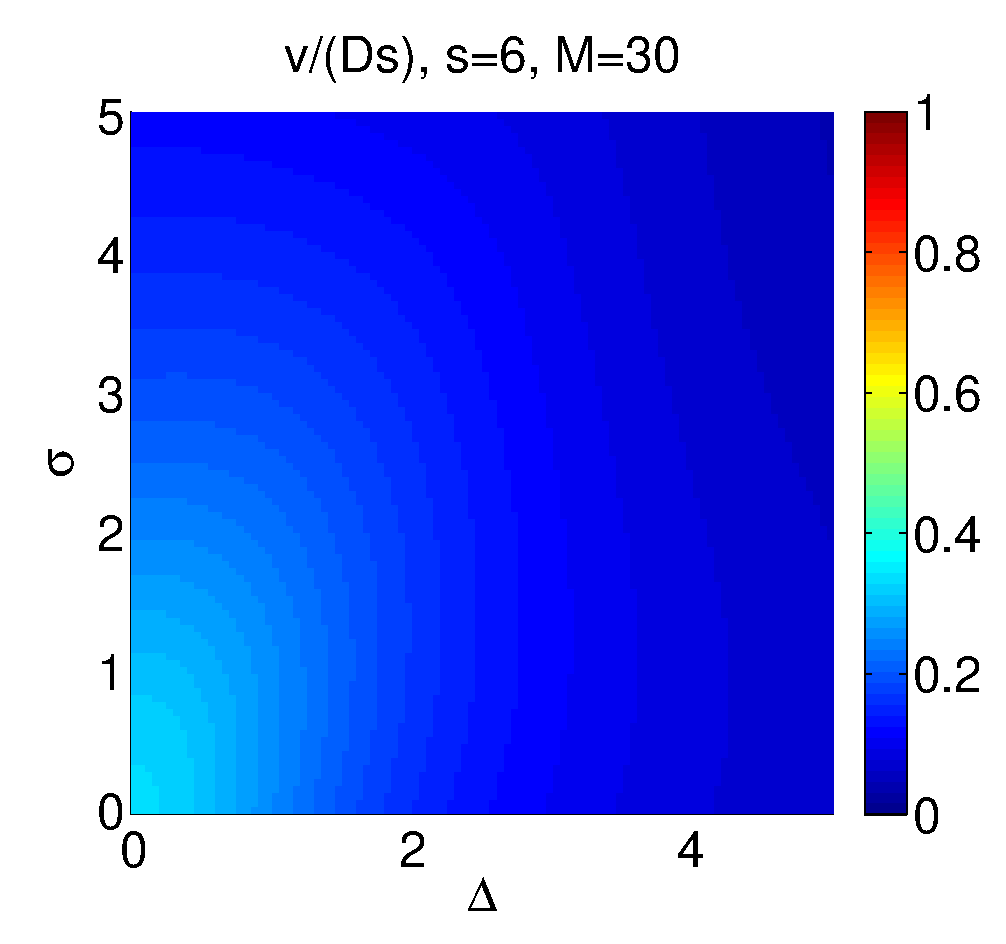
\includegraphics[height=4cm]{/Figs/vDs_4.eps}
%
%
\includegraphics[height=4cm]{/Figs/vhs_1.eps}
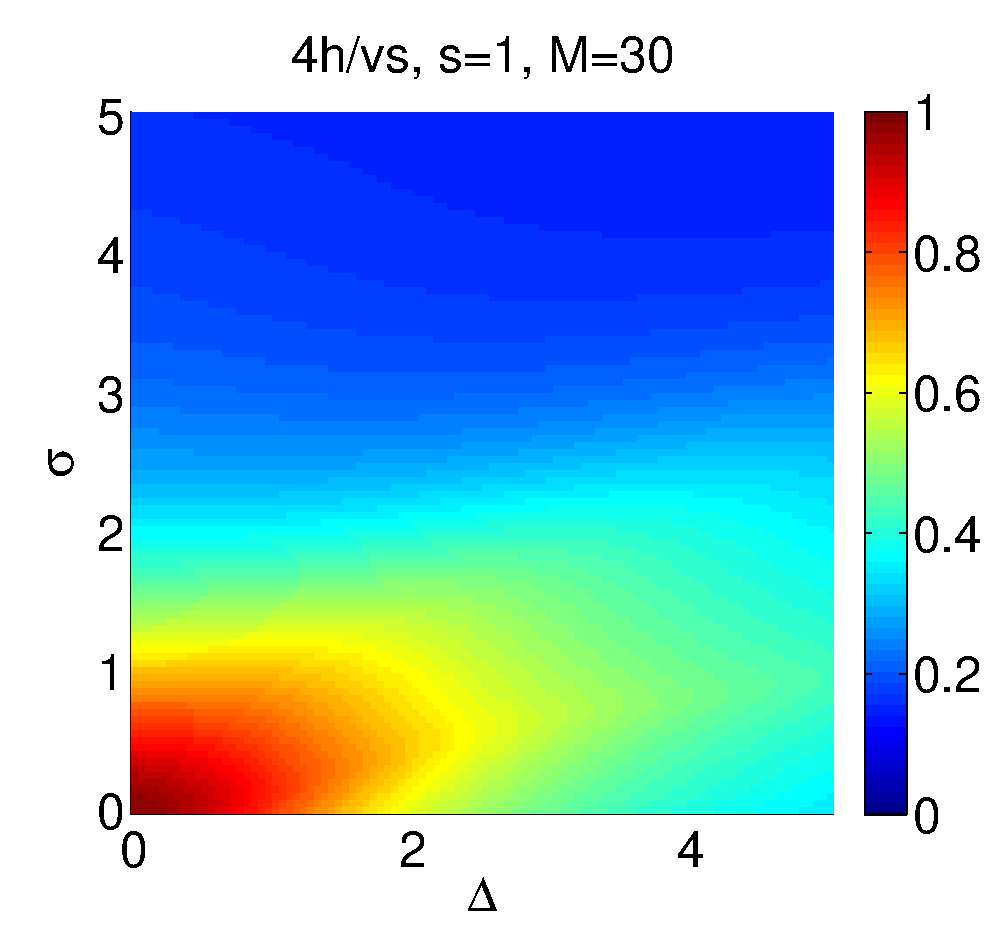
\includegraphics[height=4cm]{/Figs/vhs_2.eps}
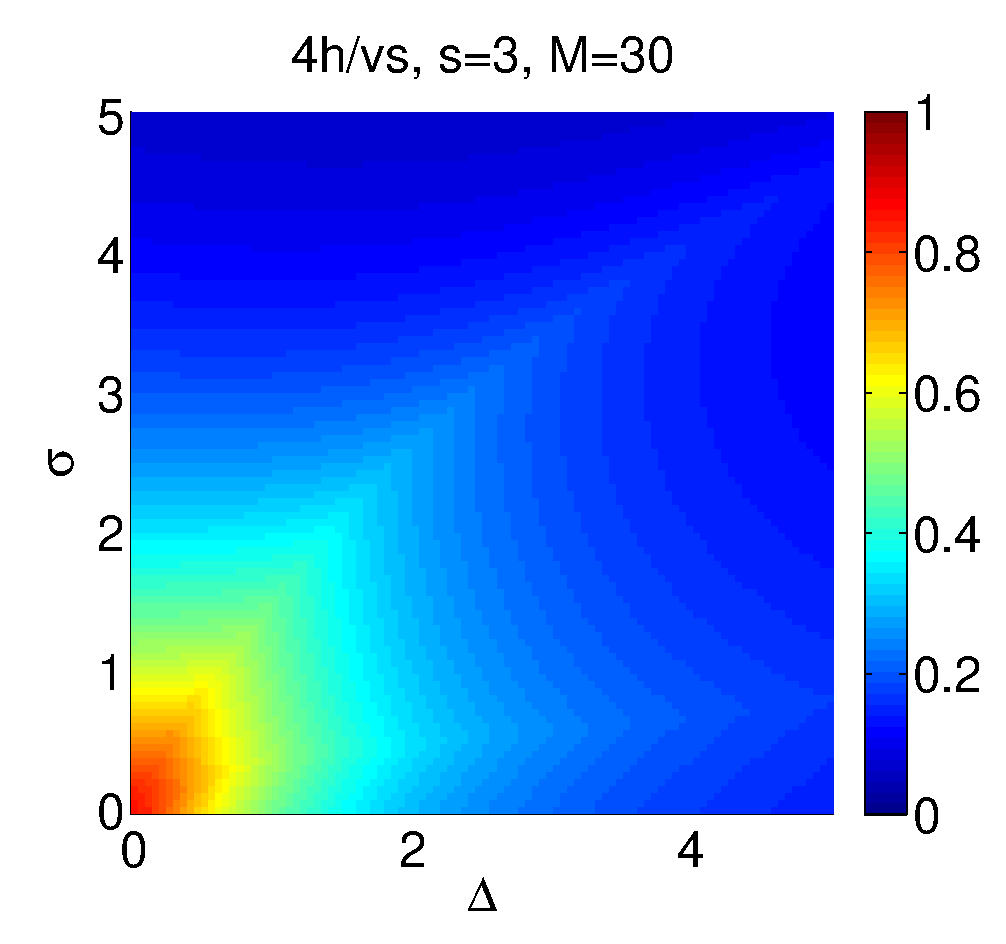
\includegraphics[height=4cm]{/Figs/vhs_3.eps}
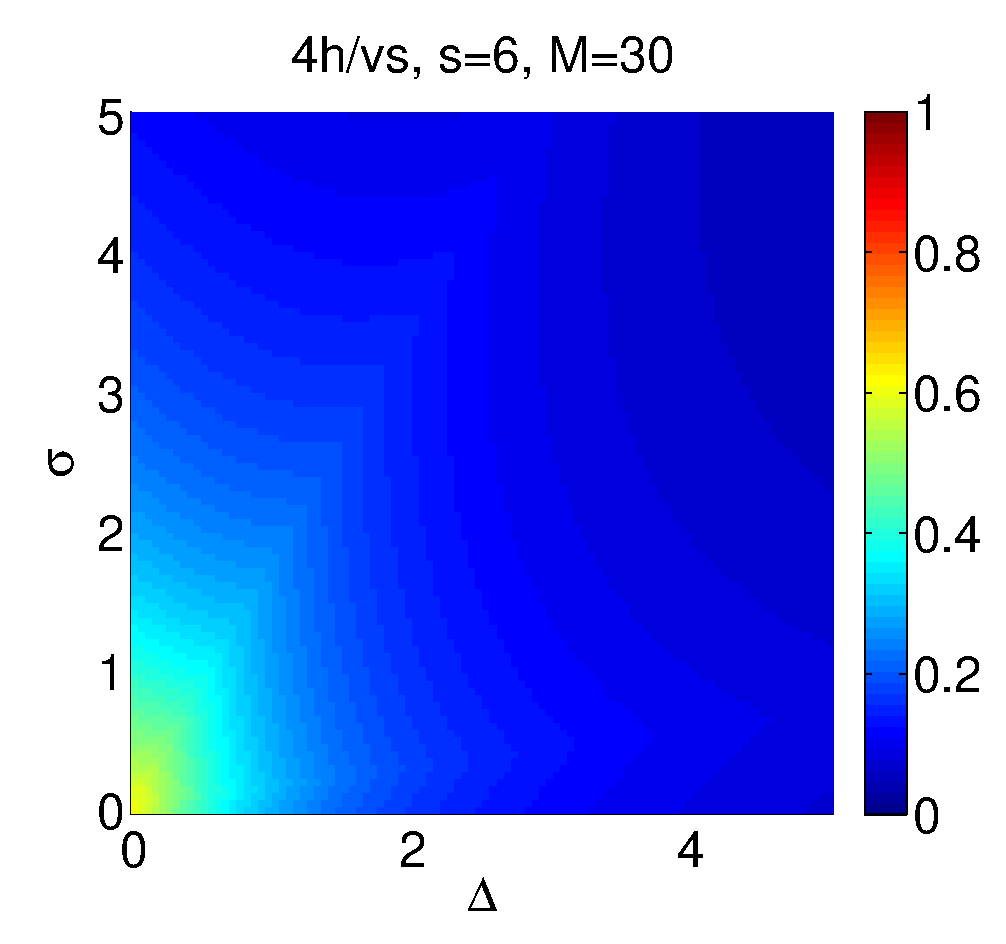
\includegraphics[height=4cm]{/Figs/vhs_4.eps}

\caption{
The measures for Gaussian statistics are imaged as a function of $\Delta$ and $\sigma$ 
for representative values of $s$. }
\label{fig3}
\end{figure}
%%%%%%%%%%%%%%%%%%%%%%%%%%%%%%%%%%%%%%%%%%%%%%




\newpage 
%%%%%%%%%%%%%%%%%%%%%%
\section{The shape of $g(\lambda)$}

Given $v$ and $D$, the parabola is defined and it has a peak value of 
%
\beq
h[\text{Gaussian}] = v^2/4D
\eeq
%
In general, however, the peak value is different 
In the Poisson limit, $s\to \infty$, it is easy to show that 
the minimum of the generating function is given by the smallest transition rate
%
\beq
h[\text{Poisson}] = \text{min}[\ora{w}_n]
\eeq



If there is no disorder, the cumulant generating function can easily be shown to be 
%
\beq
g(\lambda) &=& \ora{w} \eexp{\lambda a} + \ola{w} \eexp{-\lambda a} -(\ola{w}+\ora{w}) 
\eeq
%
For zero bias ($s=0$) this reduces to
%
\beq
g(\lambda) \ =  \ 2w(\cosh(\lambda a)-1)
\eeq
%
We emphasize that even in the absence of disorder and zero bias, 
the distribution is not Gaussian, due to having a discrete lattice (\Fig{fig4}).

\ \\ \ \\ 


%%%%%%%%%%%%%%%%%%%%%
\begin{figure}[h]
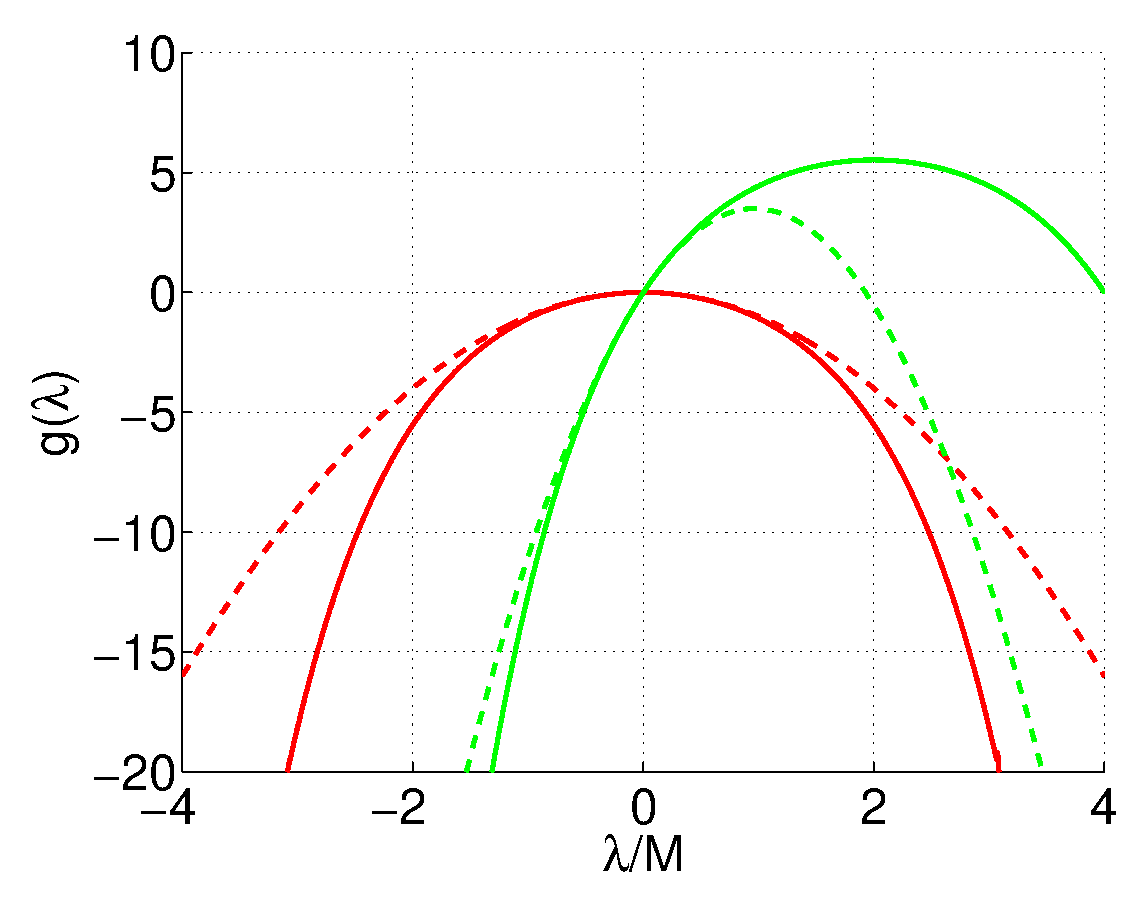
\includegraphics[height=7cm]{/Figs/g_lambda_M.eps}

\caption{The effect of discretization  on the generating function $g(\lambda)$.The red line is for $s=0$, the green line is for $s=4$. 
In both cases $\sigma=0$ and $\Delta=0$.
Dashed lines are parabolas $v\lambda - D\lambda^2$.
}
\label{fig4}
\end{figure}
%%%%%%%%%%%%%%%%%%%%%

\clearpage
%%%%%%%%%%%%%%%%%%%%%%%%%%%%%%%%%%%%%
\section{Gauging out the field disorder}
The field disorder can be removed from the off diagonals by a simple gauge transformation.
After the gauge transformation we have
%
\beq
\tilde{W} = -\text{diag}[\Gamma_{n-1}] + \text{offdiag}[ g_n e^{\pm s/2}]
\eeq
%
where $\Gamma_n = -(\ora{w}_{n+1} + \ola{w}_n)$ due to conservativity and depends on $\sigma$ and $\Delta$, but the off diagonals are now free of $\sigma$. So, surprisingly, the field disorder 
is diagonal disorder.
Note that in the gauged basis, $\tilde{W}$ is not conservative.


%%%%%%%%%%%%%%%%%%%%%%%%%%%%%%%%%%%%%%%
\section{The spectrum}
We define $\Gamma^{(s)} \equiv -\tilde{W}$, 
%
\beq
\Gamma^{(s)} &=& \text{diag}[\gamma] + \text{offdiag}[ -ge^{\pm s/2}]
\eeq
%


The eigenvalues of $\Gamma$ are solutions to the equation 
%
\beq
\det ( \Gamma^{(s) }- \varepsilon \mathcal{I})   = 0
\eeq
%
This determinant can be calculated using a formula due to Molinari. 
We define the matrix \rmrk{[check the indices... go over the convention with Doron]}
%
\beq
T^{(n)} &=& \left(
\begin{array}{cc}
 \gamma_{n-1} -\varepsilon& -g_n^2 \\
1 & 0
\end{array}
\right)
\eeq
%
where $\gamma_n$ is the escape rate of the $n^{th}$ site.
%
And obtain
\beq
\det ( \Gamma^{(s) }- \varepsilon \mathcal{I})  &=& \mathrm{tr} \left [\prod_{n=1}^N T^{(n)}  \right] - \left[\prod_{n=1}^N g_n\right]  2\cosh\left(\frac{sN}{2}\right) = \\
&=& \det  \Gamma^{(0)}  - \left[\prod_{n=1}^N g_n\right]   2\left(\cosh\left(\frac{sN}{2}\right) -1\right)= \\
&=& \prod_{j=1}^N (\varepsilon - \varepsilon_j^{(0)}) -  \left[\prod_{n=1}^N g_n\right]  2\left(\cosh\left(\frac{sN}{2}\right) -1\right)
\eeq
%
Where $\Gamma^{(0)}$ means that on the off diagonals we set $s=0$, but do not touch the diagonal.
So, in fact the eigenvalues $\varepsilon_j^{(0)}$ depend on $s$.
According to Thouless, for the corresponding Hermitian problem
%
\beq
e^{\kappa N} = \prod_{j=1}^N{\frac{  (\varepsilon - \varepsilon_j^{(0)}) }{  w_j }}
\eeq
%
where $\kappa = 1/\xi$ is the inverse localization length.
In order for $\epsilon$ to be an eigenvalue of $\Gamma^{(s)}$, it must be a solution to the equation 
%
\be{61}
\sum_{j=1}^N \left[ \log \left(\frac{\varepsilon - \varepsilon_j}{w_j}\right)\right] =
 \log \left[2\left(\cosh\left(\frac{sN}{2}\right) -1\right)\right] 
\ee
%
The left hand side oscillates and the right hand side is a straight line. 
The number of intersections is the number of real eigenvalues, see \Fig{fig5}
%%%%%%%%%%%%%%%%%%%%%%%%%%%%%%%%%%%%%%%%%%%%%%%%%%%%%%%%%%%%%%%%
\begin{figure}[h]
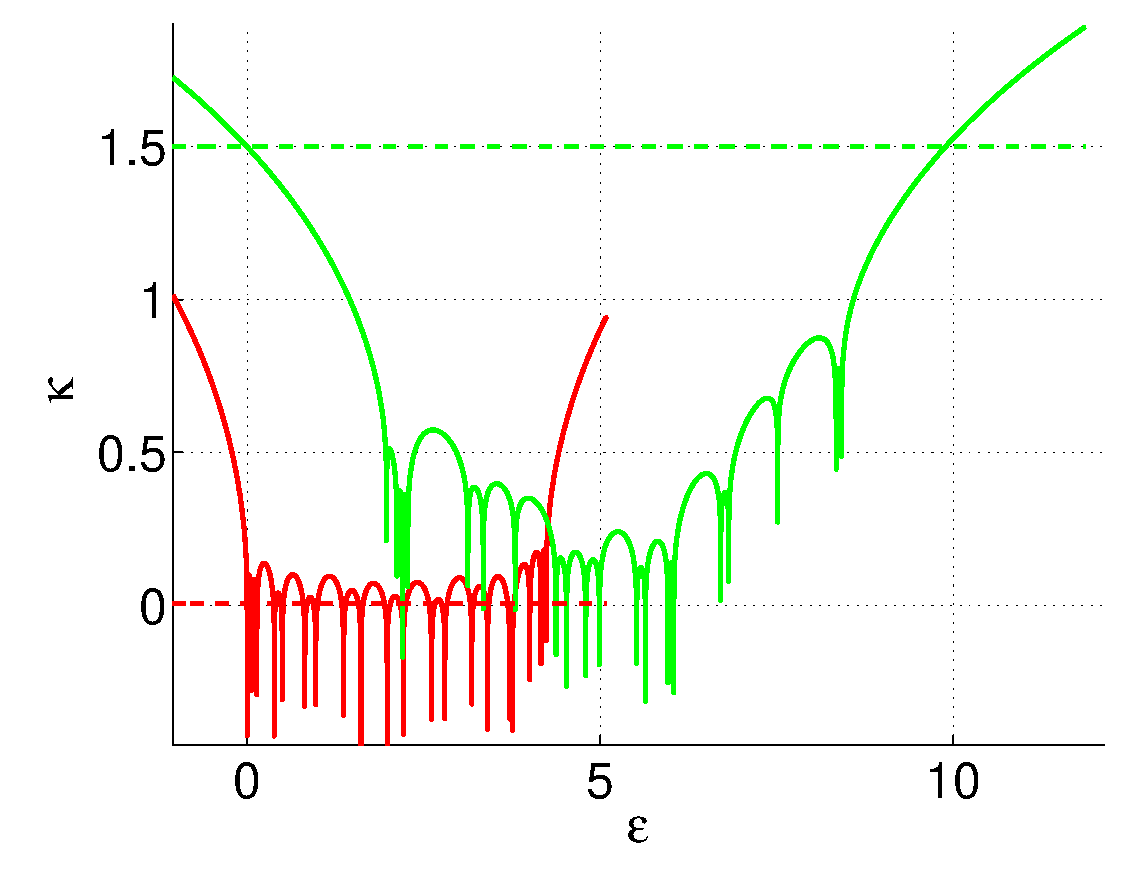
\includegraphics[height=6cm]{/Figs/kappa_1_a.eps}
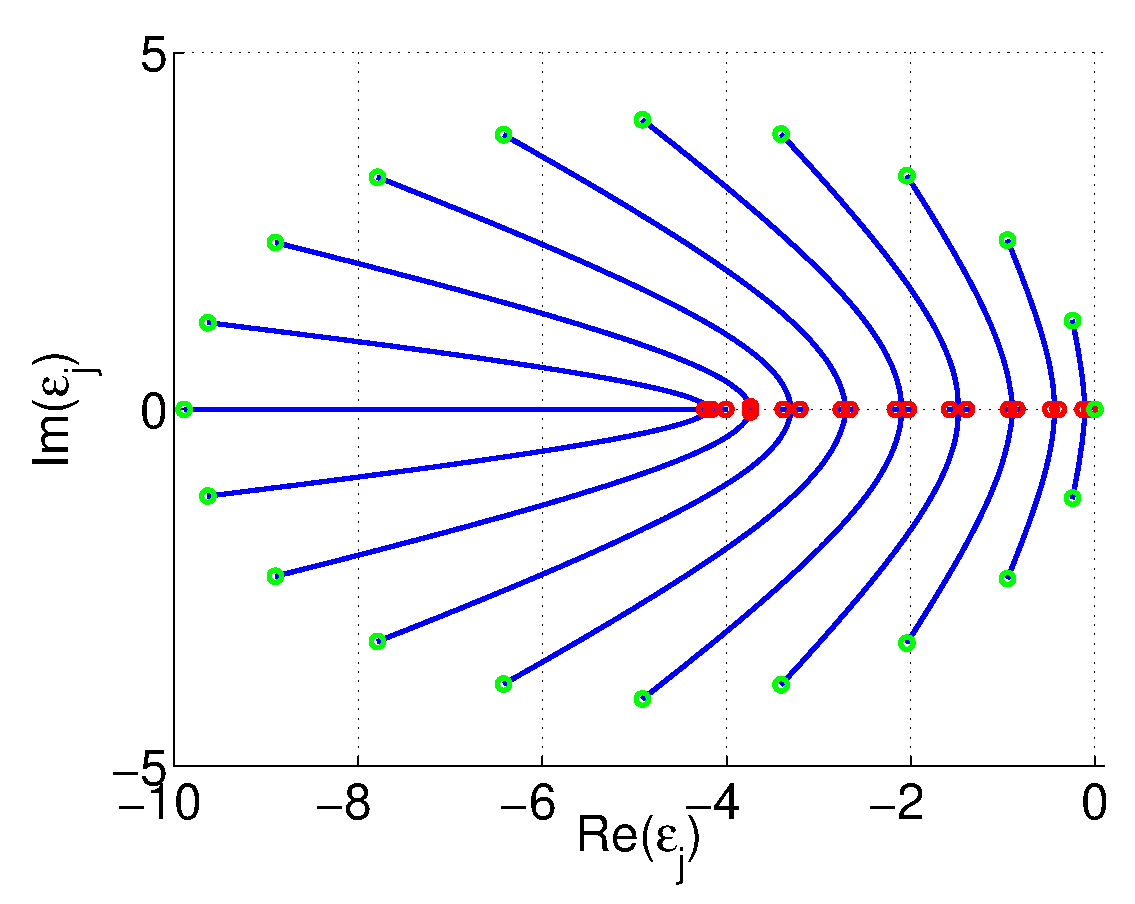
\includegraphics[height=6cm]{/Figs/epsilon_s_1_a.eps}
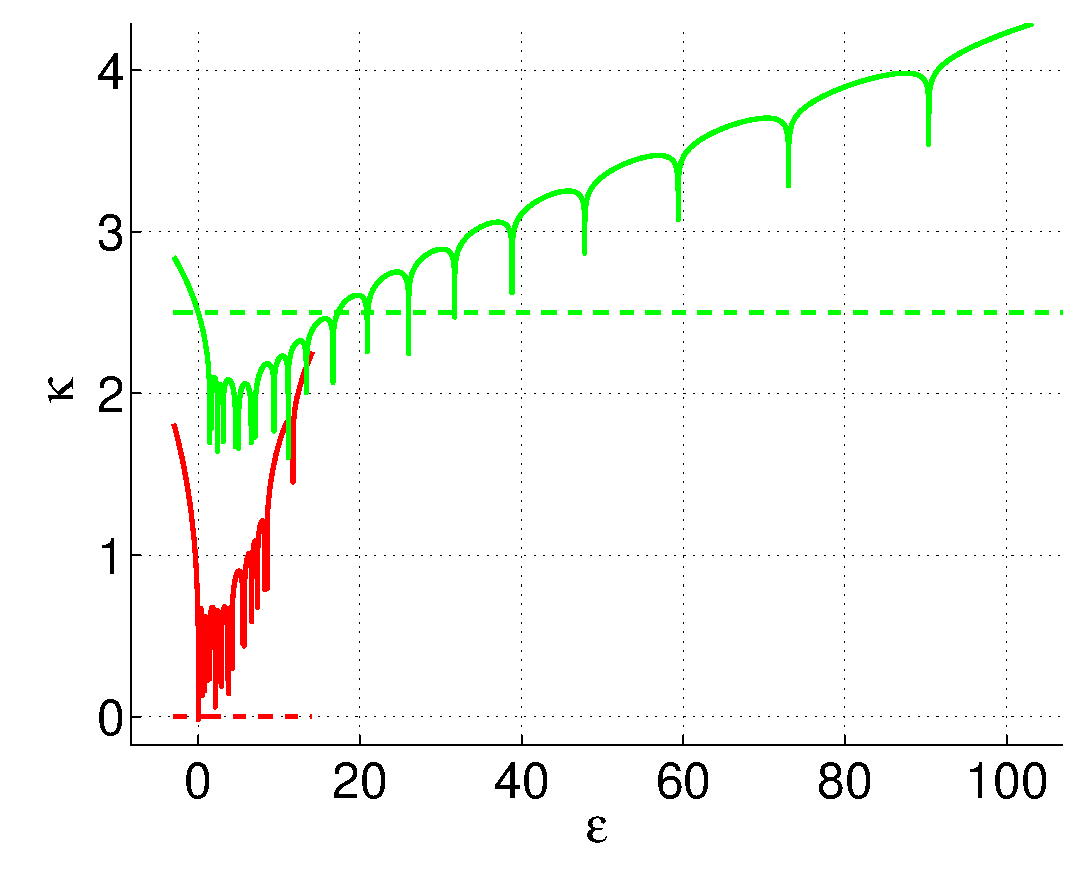
\includegraphics[height=6cm]{/Figs/kappa_2_a.eps}
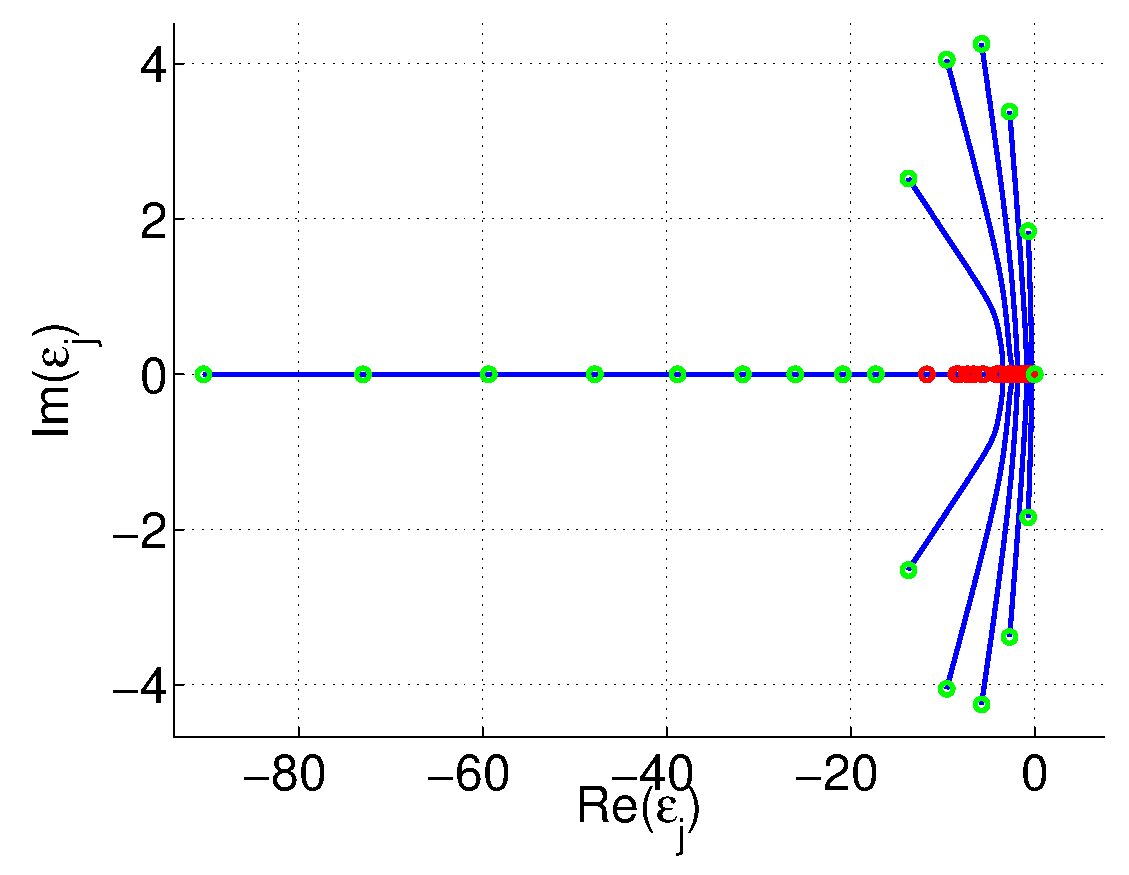
\includegraphics[height=6cm]{/Figs/epsilon_s_2_a.eps}

\caption{
Top row: The inverse localization length $\kappa$ vs. $\varepsilon$ (left panel) for ${N=20, \ \sigma=1}$, $s=0.1$ (red) and $s=3$ (green). The dashed lines are the right hand side of \Eq{e61}.
For small $s$ all eigenvalues are real, for large $s$, only two are real.
The right panel shows the trajectories of the eigenvalues  in the complex plane as $s$ is increased. 
The green and red dots correspond to the lines of the left panel.
Notice that $\varepsilon=0$ is always a solution.
Bottom row: same as top row, but here $\sigma=4$ and $s=0.1$ (red) and $s=5$ (green).
}
\label{fig6}
\end{figure}
%
In the nonconservative case, one can raise the horizontal line (right hand side of \Eq{e61}) by increasing $s$,
thus making the entire spectrum complex. 
For a conservative matrix, however, $\kappa$ is also a function of $s$, so increasing $s$ raises $\kappa$ 
more or less at the same rate, leaving the number of intersections unchanged, see \Fig{fig7}.
%
This claim can be seen mathematically from \Eq{e61}.
Due to the conservative property, the $\sigma$ disorder is in fact diagonal disorder. Therefore, for large enough $s$, the eigenvalues of the "symmetrized" martix, $\varepsilon_j^{(0)}$ grow proportialy to $\exp (s)$. 
Increasing $s \to s+\Delta s$, we have
%
\beq
\sum_{j=1}^N \left[ \log \left(\frac{\varepsilon - \varepsilon_j e^{\Delta s}}{w_j}\right)\right] &=&
 \log \left[2\left(\cosh\left(\frac{(s+\Delta s)N}{2}\right) -1\right)\right] \\
\sum_{j=1}^N \left[ \log \left(\frac{\varepsilon e^{-\Delta s} - \varepsilon_j }{w_j}\right)\right]  + N\Delta s&=&
 \log \left[2\left(\cosh\left(\frac{sN}{2}\right) -1\right)\right] +N\Delta s\\ 
\eeq
%
But $\varepsilon$ is just a dummy variable, so we can redefine $\varepsilon \equiv \varepsilon e^{-\Delta s}$ and the equation is unchanged. Thus increasing $s$ does not change the number of complex solutions.


%%%%%%%%%%%%%%%%%%%%%%%%%%%%%%%%%%%%%%%%%%%%%%%%%%%%%%%%%%%%%%%
\begin{figure}[h]
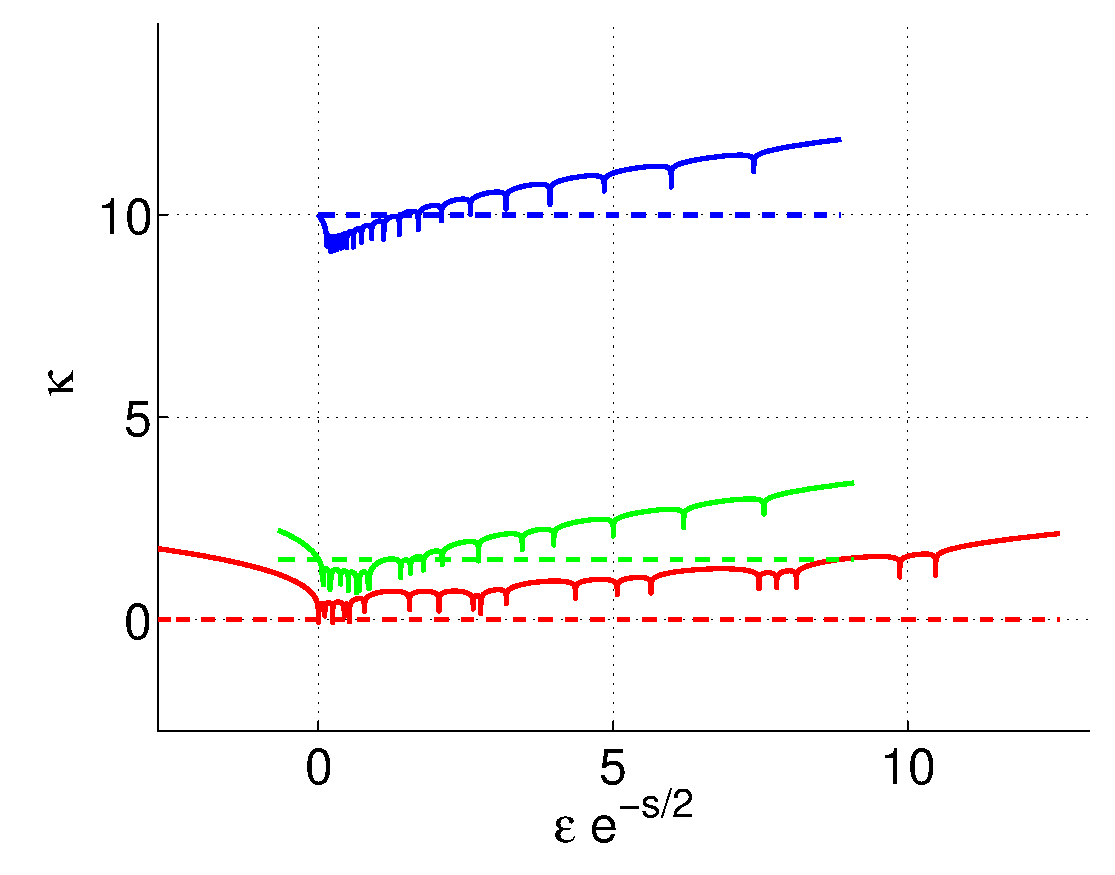
\includegraphics[height=5cm]{/Figs/kappa_4a.eps}
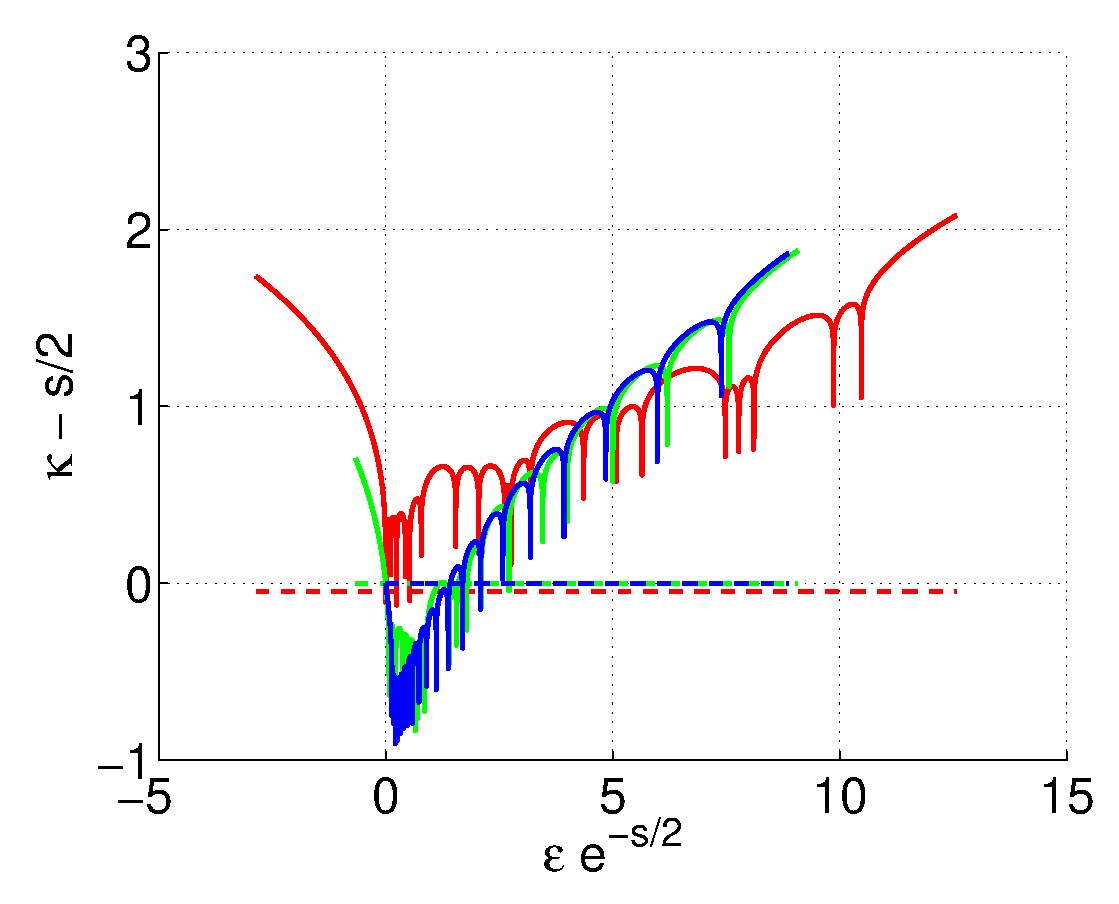
\includegraphics[height=5cm]{/Figs/kappa_4.eps}
\caption{
The inverse localization length $\kappa$ vs. $\varepsilon$ for ${N=20, \ \sigma=4, \ \Delta=0}$, $s=0.1$ (red), $s=3$ (green) and $s=20$ (blue). The dashed lines are the right hand side of \Eq{e61}.
In the right panel, the horizontal axis is $\varepsilon e^{-s/2}$ and the vertical axis is $ \kappa-s/2$.
}
\label{fig7}
\end{figure}
%


%%%%%%%%%%%%%%%%%%%%%%%%%%%%%%%%%%%%%%%%%%%%%%%%%%%%%%%%%%%%%%%%%
\section{Effect of glassiness on complexity saturation}
The effect of glassiness, or offdiagonal disorder ($\Delta$) is to further supress the complexity, however now the plateau becomes fuzzy, as seen in \Fig{fig8}. This happens because the off diagonal disorder spreads out the eigenvalues as in \Fig{fig9}.
For large $s$, the eigenvalues are approximated by the diagonal elements
%
\beq
\varepsilon_j \approx \exp \left[-B_j + \mathcal{E}_j \right] \sim \exp\left[-B_j +\frac{s}{2}\right]
\eeq

%%%%%%%%%%%%%%%%%%%%%%%%%%%%%%%%%%%%%%%%%%%%%%%%%%%%%%%%%%%%%%%
\begin{figure}[h]
\includegraphics[height=5cm]{/Figs/num_cplx_Delta.eps}
\includegraphics[height=5cm]{/Figs/num_cplx_Delta_sigma.eps}
\caption{The number of complex eigenvalues for $\Delta=1$ (red) and $\Delta=5$ (green) for $\sigma=0$ (left panel) and $\sigma = 3$ (right panel).
}
\label{fig8}
\end{figure}

%%%%%%%%%%%%%%%%%%%%%%%%%%%%%%%%%%%%%%%%%%%%%%%%%%%%%%%%%%%%%%%
\begin{figure}[h]
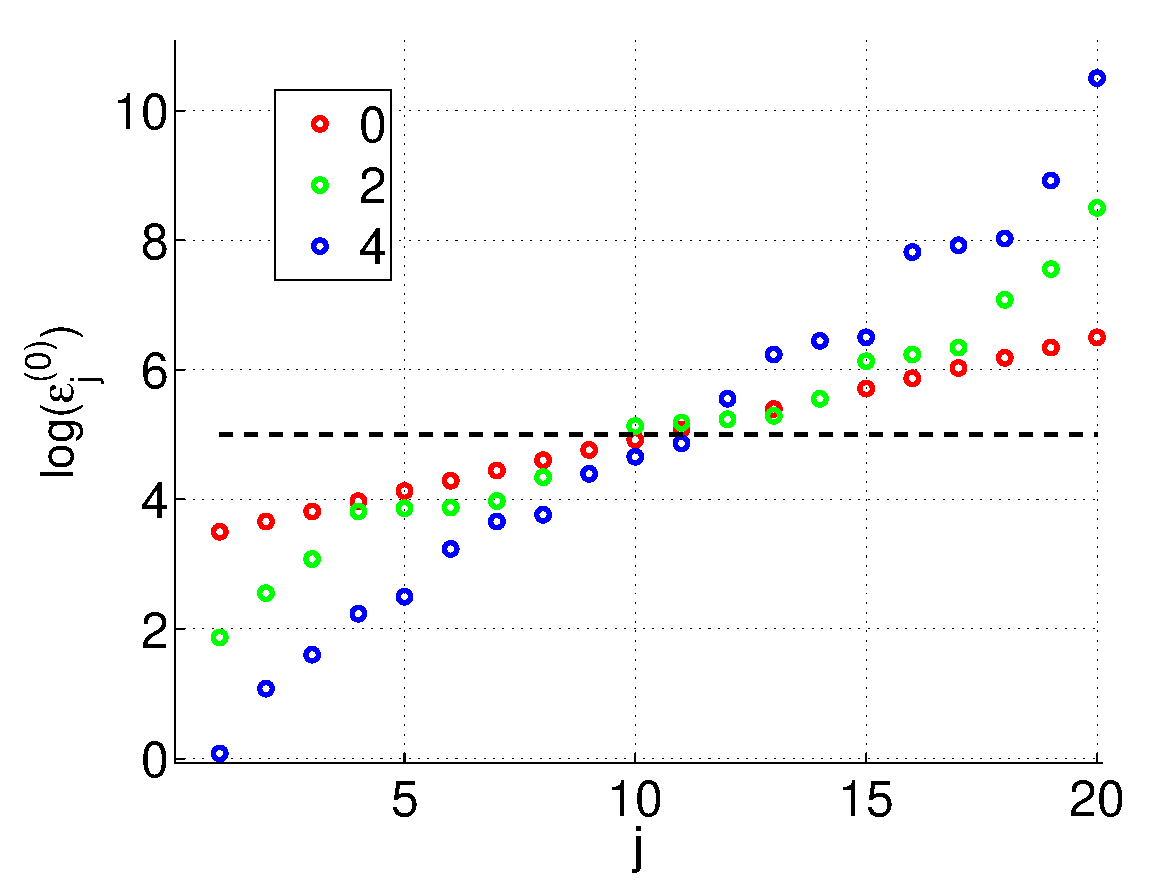
\includegraphics[height=5cm]{/Figs/epsilon_j.eps}
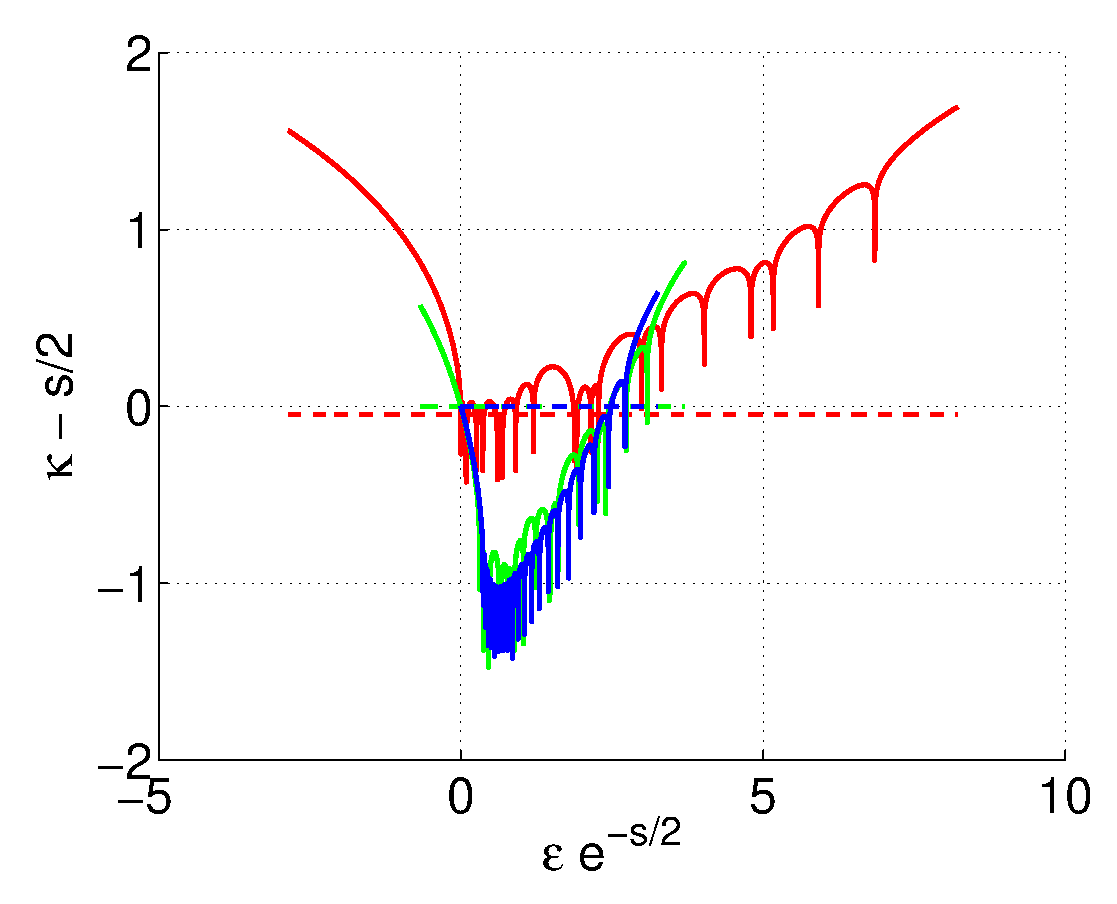
\includegraphics[height=5cm]{/Figs/kappa_Delta.eps}
\caption{The eigenvalues $\varepsilon_j^{(0)}$ for $\sigma=3$ and varying $\Delta$ (see legend). As $\Delta$ increases, the eigenvalues spread out (left panel), the dashed  black horizontal line is $s/2$. As a result, 
there are more real eigenvalues(right panel).
}
\label{fig9}
\end{figure}

%%%%%%%%%%%%%%%%%%%%%%%%%%%%%%%%%%%%%%%%%%%%%%%%%%%%%%%%%%%%%%%
\clearpage
\section{The ABAB model}
Consider the simplest model with "disorder". A lattice of period $N=2$, with transition rates 
$\ln(\ora{A}/\ola{A}) = s+\sigma$ and $\ln(\ora{B}/\ola{B}) = s-\sigma$.
The Derrida criterion is $s_c = \ln(\cosh \sigma)$

\begin{figure}[h]
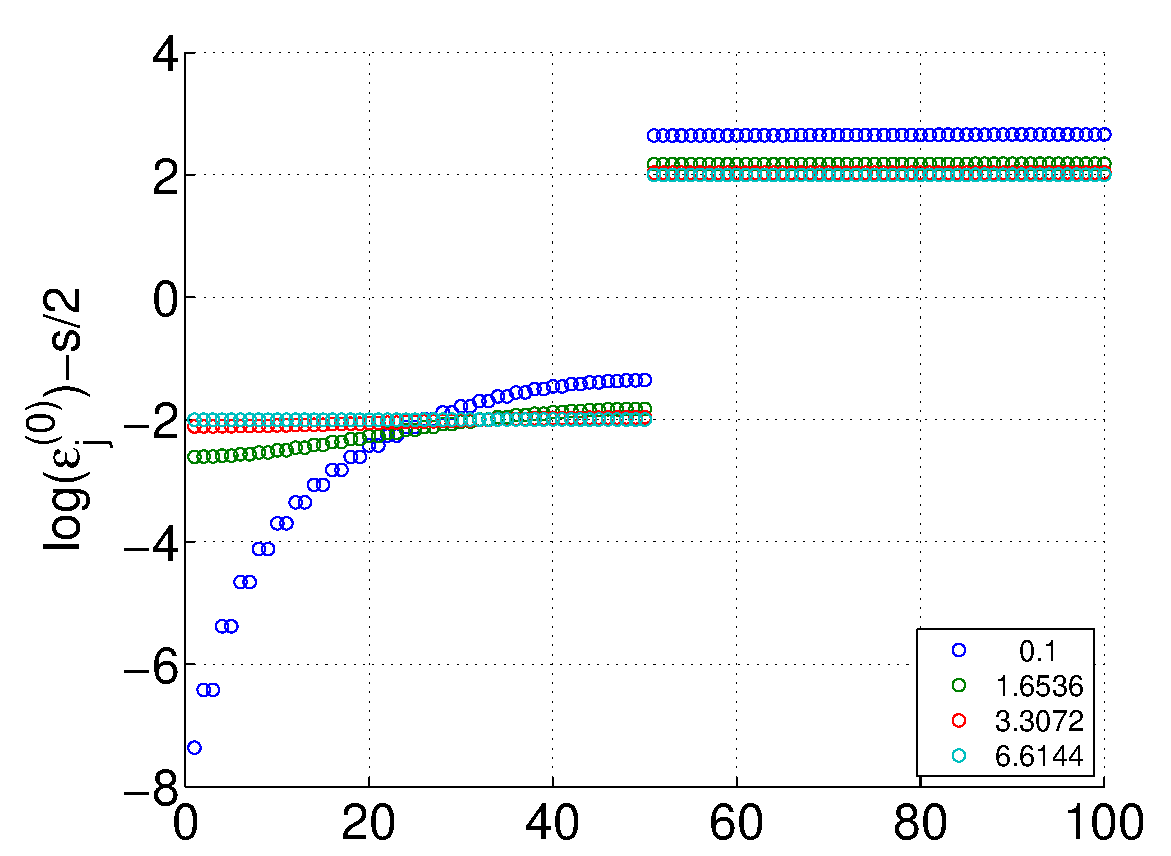
\includegraphics[height=5cm]{/Figs/epsilon_j_N_2.eps}
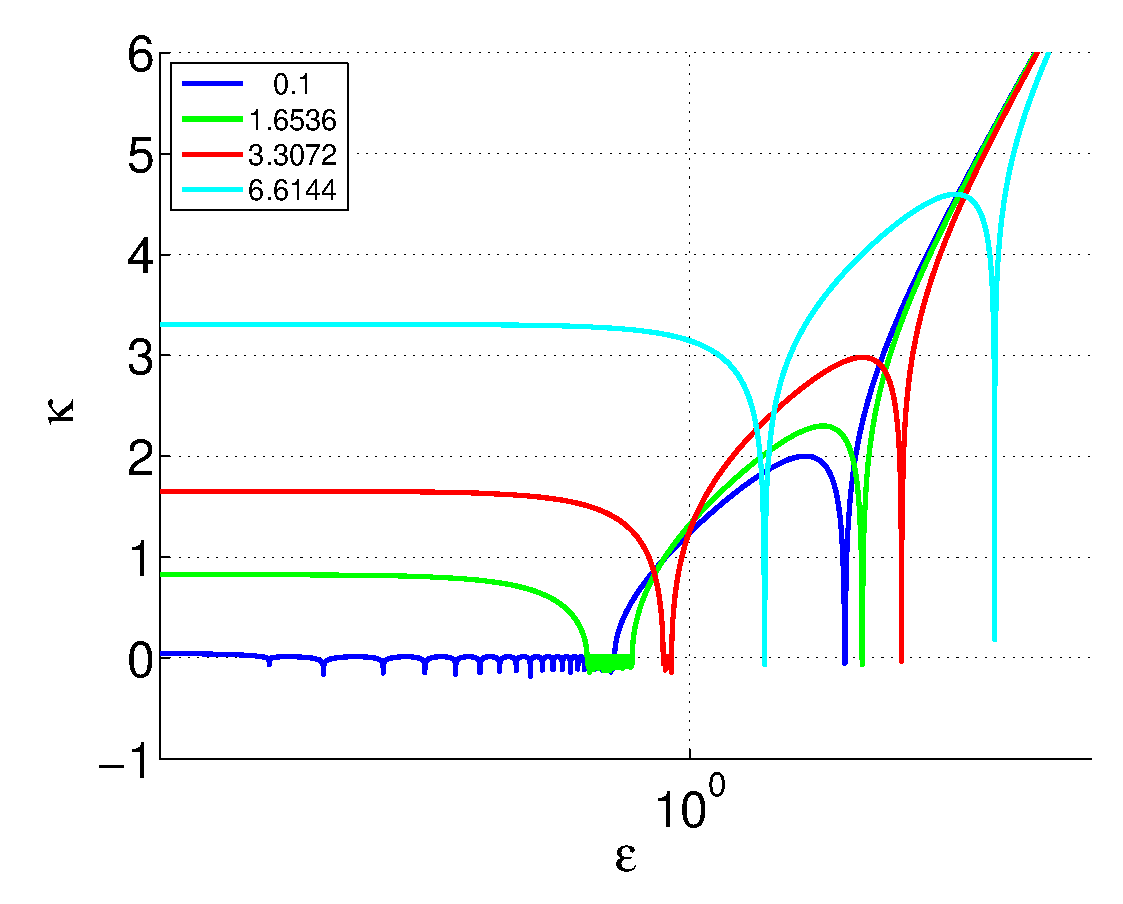
\includegraphics[height=5cm]{/Figs/kappa_N_2.eps}
\caption{The eigenvalues $\varepsilon_j^{(0)}$ (left) for $\sigma=4$ and varying $s$ (see legend)
and the inverse localisation length $\kappa$ (right)
The red line is for $s=s_c$}
\label{fig10}
\end{figure}


%%%%%%%%%%%%%%%%%%%%%%%%%%
%%%%%%%%%%%%%%%%%%%%%%%%%%%%%%%%%%%%%%%%


% complex gap , this is done by looking at how the 
%real part of the complex eigenvalues behave as $\mathcal{S}$ increases.
%Adding an imaginary part, such that $x\to x+iy$, \Eq{e9} is in fact two equations. 
%The real part is
%%
%\be{10}
%\cos (x) \left[ \cosh (y) - gy \sinh (y) \frac{x^2+y^2 - \mathcal{S}^2/4}{2(x^2+y^2)} \right]
%+\sin(x) \left[ gx \cosh(y)\frac{x^2+y^2 + \mathcal{S}^2/4}{2(x^2+y^2)}   \right]
%= \cosh\left(\frac{\mathcal{S}}{2}\right)
%\ee
%%
%We solve this equation for $x$ for various values of $y$. 
%It is evident in \Fig{fig2} that $x$ increases with $y$, 
%leading to the conclusion that any complex eigenvalue has a finite real part.
%The minimum value of $x$ determines the gap.
%%
%Thus we conclude that in this model, of a ring and a single diffusive scatterer
%there is always a gap which is due to $\mathcal{S}$.
%%%%%%%%%%%%%%%%%%%%%%%%%%%%%%%%%%%
%\begin{figure}[h]
%\includegraphics[height=5cm]{/Figs/y_x.eps}
%\caption{The first numerical solution of \Eq{e10}. The trajectory of the real part, $x$. The dashed line is $y = \mathcal{S}/2$. Here $\mathcal{S}=1$ (blue) and $\mathcal{S}=5$ (red) and $g=0.1<g_c$. The left most point of each line is the lower bound on the gap.}
%\label{fig2}
%\end{figure}


%
%\begin{figure}[h]
%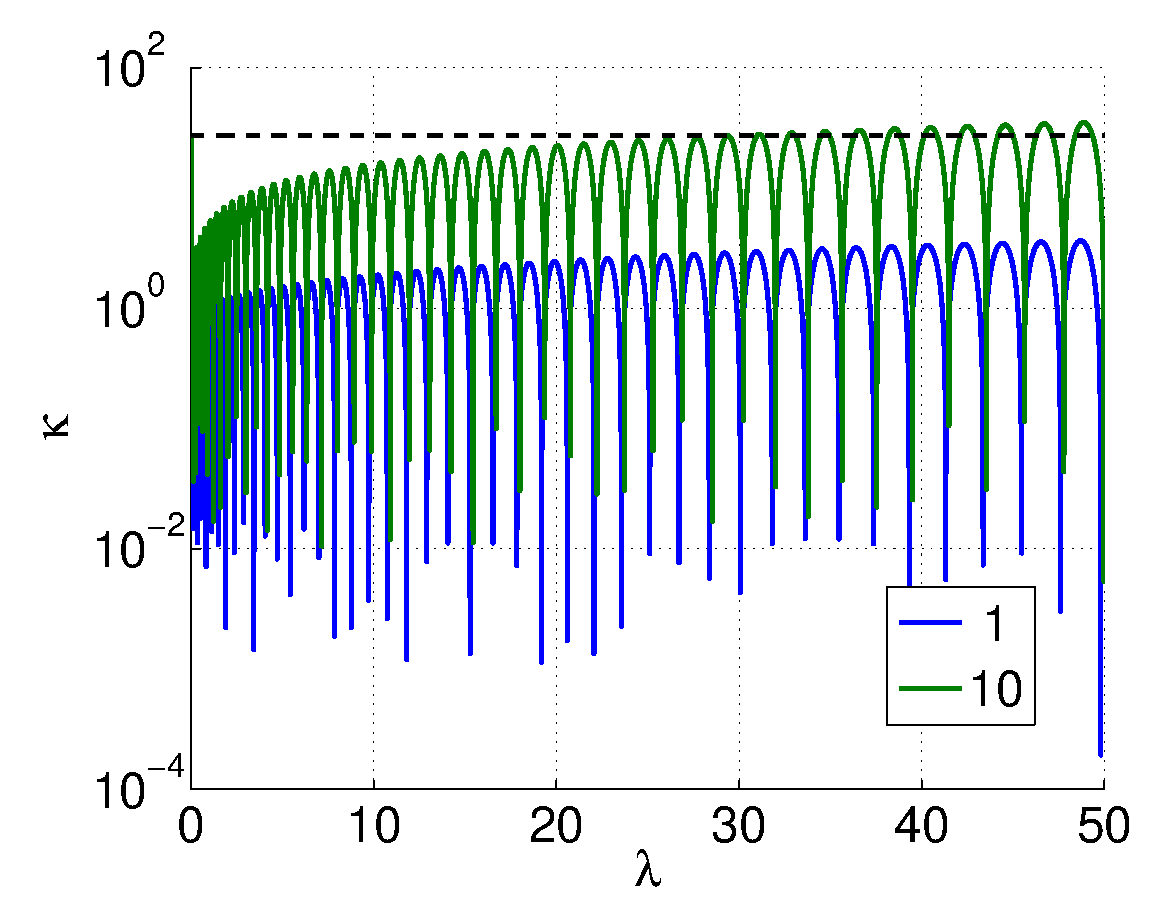
\includegraphics[height=5cm]{/Figs/kappa_nhr.eps}
%\caption{The l.h.s of \Eq{e7} for $\alpha=1$ and $\alpha=10$, $L=20, \ s=0.4$. }
%\end{figure}

%%%%%%%%%%%%%%%%%%%%%%%%%%%%%%%%%%%%%%%%%%%%%%%%%%
\clearpage
\section{Observations}
The disordered model shows some very interesting behaviour. 
We present here our main observations.

%%%%%%%%%%%%%%%%%%%%%%%%%%%%%%%%%%%%%%%%
\subsection{Complexity saturation and the sliding transition }
It is known from Derrida that there is a sliding transition where the velocity exhibits a phase transition from 
$v=0$ to finite $v$. This transition occurs at the value of $s$ for which
%
\beq
\left\langle \left( \frac{\ora{w}}{\ola{w}}\right) \right\rangle = 1
\eeq
%
This transition has fingerprints on the spectrum.  Below we plot the number of complex eigenvalues 
as a function of $s$. 
An interesting observation is that not all of the eigenvalues become complex. 
This effect is due to the conservativity, as we shall explain.
We call this "complexity saturation".
The question to answer is why this occurs at the sliding transition?
The sliding transition is dictated by the behavior of the lowest eigenvalue, however we see the fingerprint clearly across the entire spectrum.
%%%%%%%%%%%%%%%%%%%%%%%%%
\begin{figure}[h]
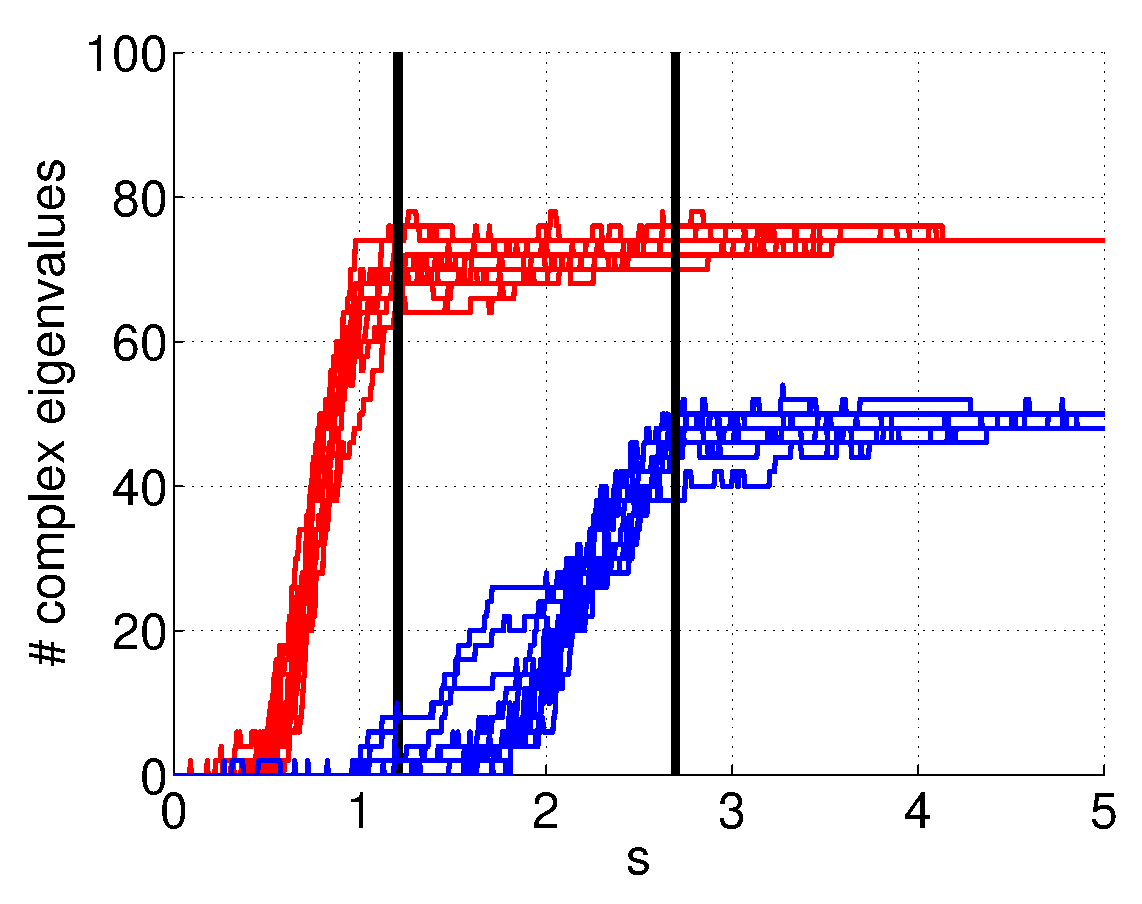
\includegraphics[height=7cm]{/Figs/num_cplx.eps}

\caption{Number of complex eigenvalues vs. $s$ for $N=100$ sites. Each red line corresponds to a different 
realisation of field disorder with $\sigma=3$(red) and $\sigma=5$ (blue), but $\Delta=0$. The black vertical lines are at values of $s$ at which the sliding transition occurs.}
\label{fig5}
\end{figure}


%%%%%%%%%%%%%%%%%%%%%%%%%%%%%%%%%%%%%%%
%%%%%%%%%%%%%%%%%%%%%%%%%%%%%%%%%%%%%%%%
\subsection{The gap}
The gap $\Delta$ in the spectrum is just the real part of the second largest eigenvalue.
Our goal is to characterise the gap for the general disordered hopping model, see for example \Fig{fig11}, where plot the gap vs. the disorder $\sigma$ and vs. the affinity $s$. 
We would like to know wether the gap closes, or grows and wether the gap is complex or not. 
When keeping $s$ and varying $\sigma$, we observe a peak in the gap at the sliding transition point, after which the gap begins to close exponentially in $\sigma$. 
%
The sliding transition occurs at (Derrida)
%
\beq
s= \log\left( \frac{\sinh \sigma}{\sigma}\right)
\eeq
%
So, by setting $s$, we can calculate numerically $\sigma_c$.
%%%%%%%%
\begin{figure}[h]
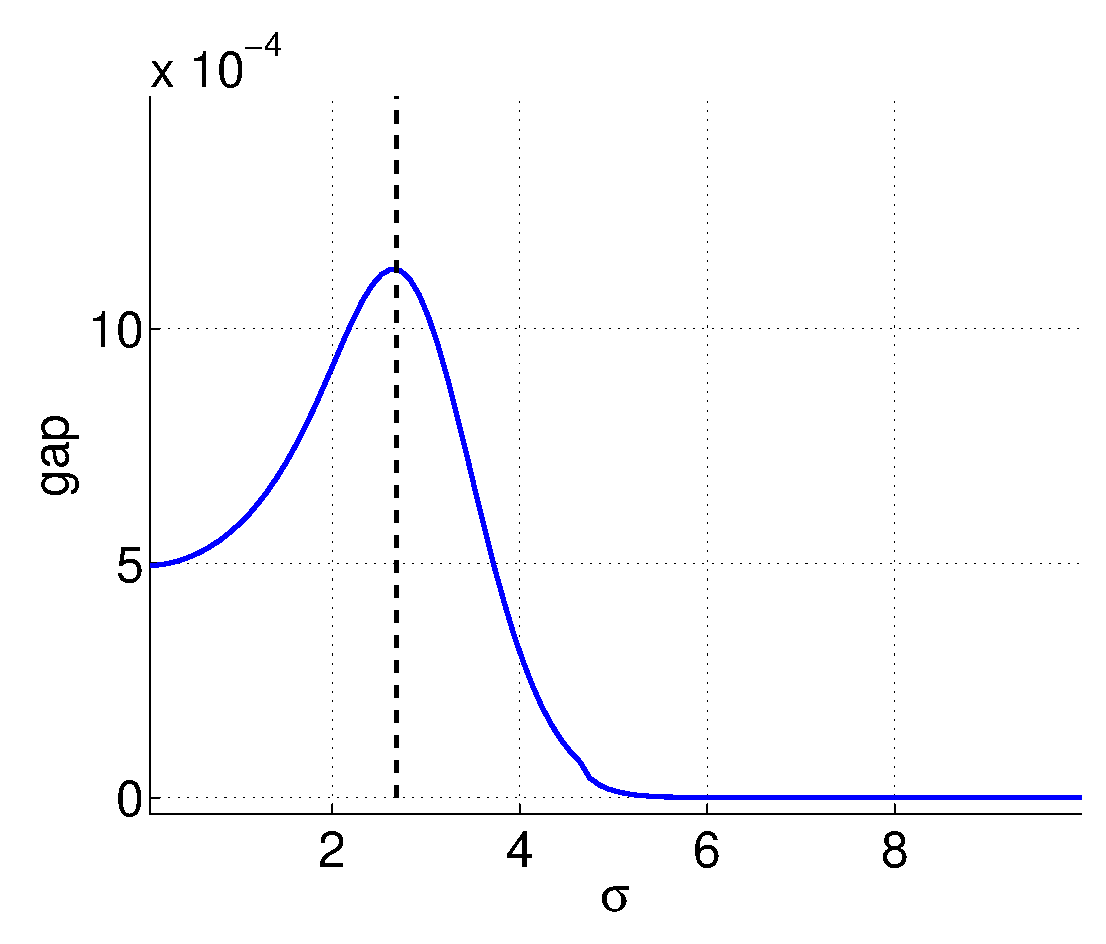
\includegraphics[height=5cm]{/Figs/gap_sigma.eps}
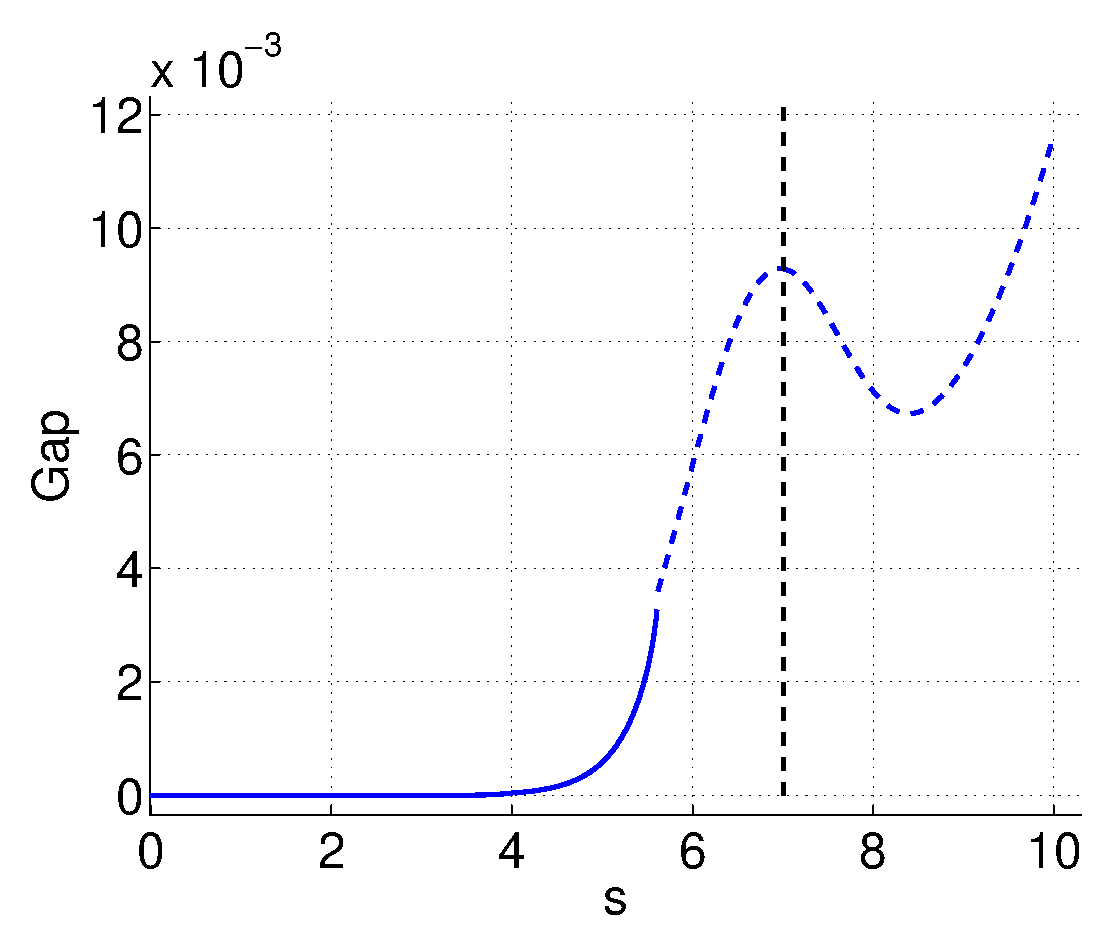
\includegraphics[height=5cm]{/Figs/gap_s_sigma_10.eps}
\caption{
Left panel: The gap in the spectrum vs. the field disorder $\sigma$ (left panel) for fixed $s$. 
At $\sigma=\sigma_c$ the gap begins to close exponentially in $\sigma$. The value $\sigma_c=2.69$ (dashed black line) is determined by the Derrida transition. Here $N=300$ and $s=1$.
Right panel: the gap in the spectrum vs. $s$.
At $s=s_c$ (dashed black line)  the gap begins to close. This point is determined by the Derrida transition. Here $N=300$ and $\sigma=10$. Dashed lines indicate that the gap is complex.}
\label{fig11}
\end{figure}
%%%%%%%%%%%%%%%%%%%%

%%%%%%%%%%%%%%%%%%%%%%%%%%%%%%%%%%%%%%%%%
\section{Continuous model}
To explain the observations we first consider three simpler continuous models of a ring of circumference $L$.
In the continuous version, the dynamics is describes by a diffusion equation with a drift term. 
%
\be{1}
\frac{\partial \psi}{\partial t} = \frac{\partial}{\partial x} \left[ D(x) \frac{\partial \psi}{\partial x}\right] -
 \frac{\partial}{\partial x} \left[v(x)\psi\right]
\ee
%
Assuming that $D(x)$ and $v(x)$ are piecewise,the 
solution to the diffusion equation in each region is  simply  $\psi \sim e^{-\lambda t + ikx}$, inserting this in \Eq{e1}, we obtain the dispersion relation 
%
\beq
\lambda &=& Dk^2 + ivk\\
k_{\pm} &=& \frac{-iv \pm \sqrt{4\lambda D -v^2}}{2D} = \frac{-is}{2} \pm \sqrt{\frac{\lambda}{D}-\frac{s^2}{4}}
\eeq
%
So, in each region the solution to \Eq{e1} has the form 
\be{2}
\psi(x) = Ae^{ik_{+} x}+ Be^{ik_{-} x} = \eexp{\frac{v}{2D}x} \left(Ae^{i\frac{\sqrt{4\lambda D -v^2}}{2D}x}+Be^{-i\frac{\sqrt{4\lambda D -v^2}}{2D}x}\right)
\ee
%
There are three limiting cases which are of interest.
In the simplest case of periodic boundary conditions and $u=0$, the eigenvalues are simply
%
\be{3}
\lambda  = Dk^2 =D\frac{4\pi^2 n^2}{L^2} \ , \ n=0,1,2,...
\ee
%
If there is a drift term, $u\neq 0$ (this is model I), the eigenvalues are 
\be{4}
\lambda &=&  D\frac{4\pi^2 n^2}{L^2}+i\frac{2\pi v}{L} n \ , \ n=0,1,2,...\\
\lambda &=&  \frac{v^2}{4D}
\ee
%
If the ring is disconnected at a point, then we have a chain and Neumann boundary conditions apply, 
leading to the eigenvalues 
%
\be{5}
\lambda &=& D\frac{\pi^2 n^2}{L^2} + \frac{v^2}{4D} \ , \ n=0,1,2,...\\ 
\lambda &=& 0
\ee
%
\subsection{The models}
\begin{enumerate}
\item
The first model is a clean ring,  with zero disorder such that that  $D(x)=D$ and $u(x)=u$. 
It is straightforward to obtain the spectrum of \Eq{e4}.
%
The gap is constant and "complex". 
%
\item
In the second model we have a ring with uniform drift velocity $u$and a diffusive scatterer,
such that the diffusion coefficient within a small region is smaller than the diffusion coefficient elsewhere. 
%
\beq
D(x) = \left\{ \begin{array}{cc}
D_0, & |x|<a/2 \\
D, & |x|>a/2 
\end{array}
\right.
\eeq
%
This is equivalent to having $g<1$ on one of the bonds in the tight binding model.
The gap is real and increasing and then becomes complex. 
Notice that in the limit $D_0\to 0$, we have a disconnected ring, corresponding to \Eq{e5}.
%
\item
In the third model, the ring is divided in to two halves. Each half of the ring has a different drift velocity,
%
\beq
v(x) = \left\{ \begin{array}{cc}
v_1 \ =\  D(s+\sigma), & 0< x<L/2 \\
v_2 \ = \ D(s-\sigma)\ , & L/2<x<L
\end{array}
\right.
\eeq
%
In the tight binding model, this is equivalent to having $\mathcal{E}_n = s+\sigma$ if $n<N/2$ 
and $\mathcal{E}_n = s-\sigma$ if $n>N/2$. 
Here the gap is initially real and decreasing until $s=\sigma$, from which point the gap becomes constant and complex.
\end{enumerate}
%
Since we are interested in the lower bands, the tight binding model provides a good approximation 
and it is very easy to obtain numerical results.
However, one must take care to take a large enough system and notice that $s$ is not too large (as illustrated by \Fig{fig4}).
The gaps,  $\Delta(s)$ for the tight binding equivalent of these three models are shown in \Fig{fig12}.

%%%%%%%%%%
\begin{figure}[h]
%\includegraphics[height=5cm]{/Figs/gap_s_I_II_III_N_100_2.eps}
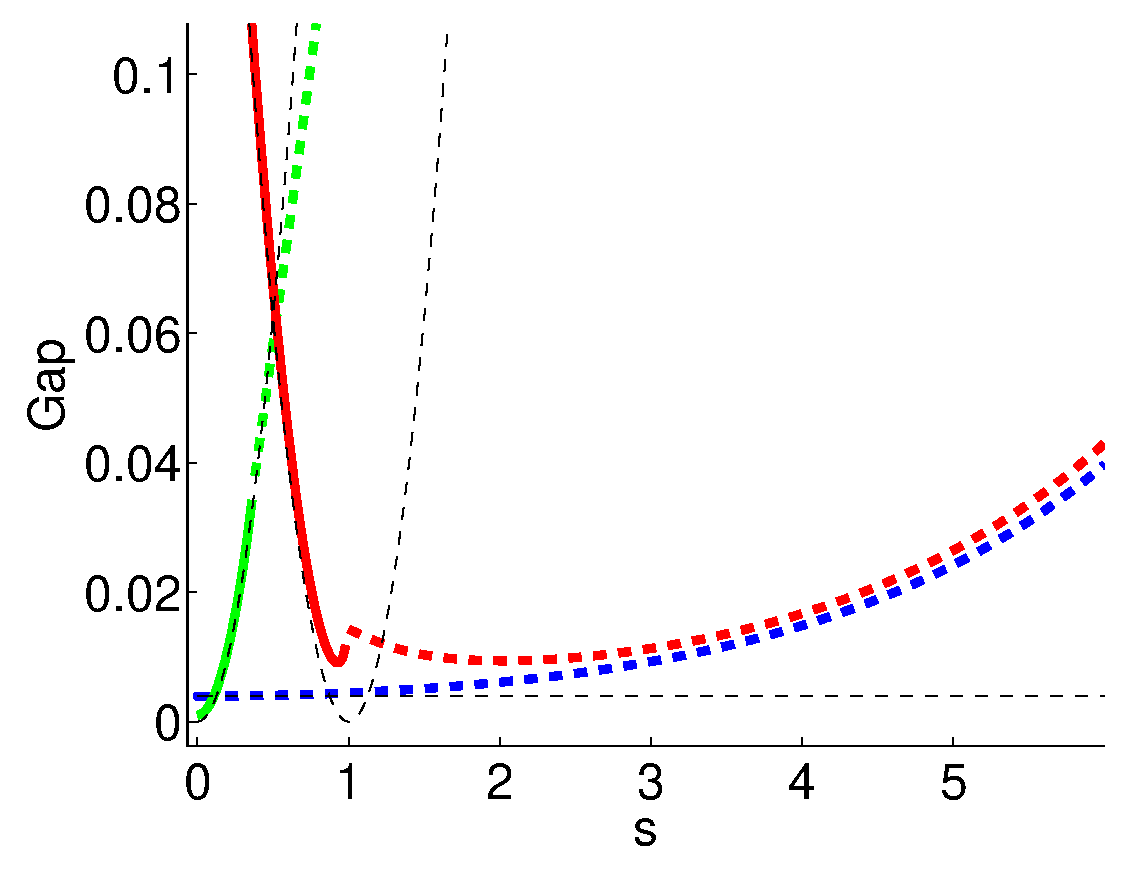
\includegraphics[height=5cm]{/Figs/gap_s_I_II_III_N_100_4.eps}
\caption{The gap in the spectrum vs. the affinity $s$ for models I (blue) ,II (green) and III (red) as described in the text. 
Here $N=100$. Solid lines indicate that the gap is real, dotted lines indicate the gap is complex. 
For model I (blue) we have $\sigma=0$ and $g=1$. For model II (green) we have $\sigma =0$ and $g=10^{-8}$. For model III (red) we have $\sigma = 1$ and $g=1$.
The horizontal black line is $\lambda=4\pi^2/N^2$, the black dotted parabolas  $s^2/4$ and $(s-\sigma)^2/4$.
\rmrk{I do not understand why $v^2/4D$ doesn't show up in the tight binding model...}
}
\label{fig12}
\end{figure}


%%%%%%%%%%%%%%%%%%%%%%%%%%%%%%%%%%%%%%%%%%%%%%
\subsection{Model II - Diffusive scatterer}
The eigenvalues are given by solutions to the secular equation.
The details of the derivation of this equation are given in the appendix.  
%
It is convenient to define the following dimensionless variables 
%
\beq
g \ & \equiv & \ \frac{\alpha D}{L} \ \ = \ \ \frac{a}{L}\cdot \frac{D}{D_0} \\
z \ & \equiv & \ \tilde{k}L \ \ , \ \ \mathcal{S} \equiv sL \\
\lambda \ &=& \ D\left( \tilde{k}^2 + \frac{s^2}{4}\right)
\eeq
%
with which the  secular equation 
%
\be{9}
\cos \left(L \sqrt{\frac{\lambda}{D}- s^2/4} \right)
%
+\frac{1}{2} g \frac{\lambda}{\sqrt{\frac{\lambda}{D}-s^2/4}}\sin \left(L\sqrt{\frac{\lambda}{D}- s^2/4}\right) = \cosh\left( \frac{sL}{2}\right)
\ee
%
becomes 
%
\beq
 \cos(z) + g \frac{z^2+(\frac{\mathcal{S}}{2})^2}{2z}\sin(z)= \cosh \left(\frac{\mathcal{S}}{2} \right)
 \eeq
 %
This is a transcendental equation for $\lambda$ which we shall write as 
%
\beq
f(\lambda;\mathcal{S}) \ \ = \ \ \cosh \left( \frac{\mathcal{S}}{2} \right)
\eeq
%
In general, $\lambda$ is complex. 
The functions $f(\lambda)$ oscillates within an envelope
%
\beq
\kappa &=& \sqrt{1+ \frac{g^2\lambda^2 }{\frac{4\lambda}{D}-s^2}} \ \ = \ \ \sqrt{1+\left(g \frac{x^2+(\frac{\mathcal{S}}{2})^2}{2x} \right)^2}
\eeq
%
Real values of $\lambda$ are possible as long as $\kappa \geq cosh(\mathcal{S}/2)


which has a minimum value at $x_{min}  =   \mathcal{S}/2$ for which $f(\lambda_{min} = Ds^2/2) =1+g\mathcal{S}/2$.
When the envelope is beneath $\cosh(\mathcal{S}/{2})$ the spectrum is entirely real , otherwise it 
can be complex. The critical value $\mathcal{S}_g$ is the solution to the equation
%
\beq
1+ \frac{1}{2} g \mathcal{S} =  \cosh \left(\frac{\mathcal{S}}{2}\right)
\eeq
%
This is illustrated in \Fig{fig_f}.
%
%%%%%%%%%%%%%%%%%%%%%%%%%%%%%%%%%%%
\begin{figure}[h]
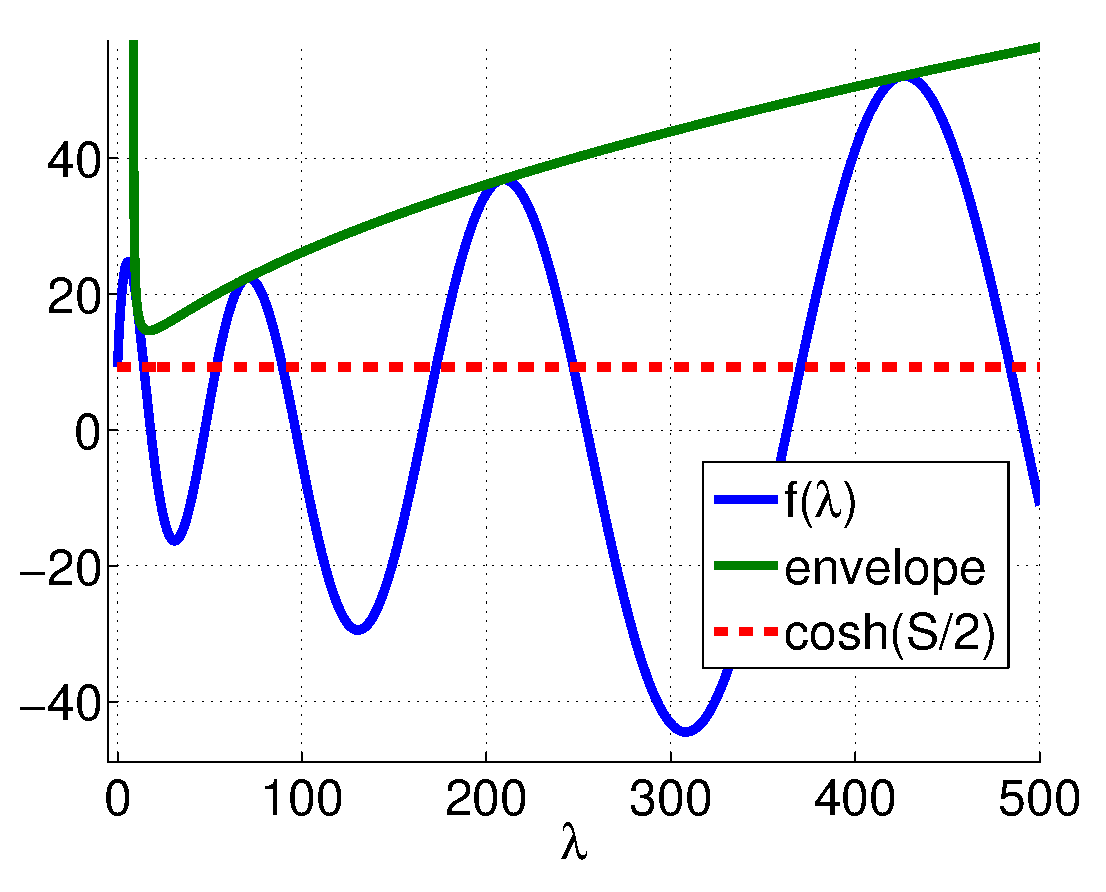
\includegraphics[height=4cm]{f_sg_m.eps}
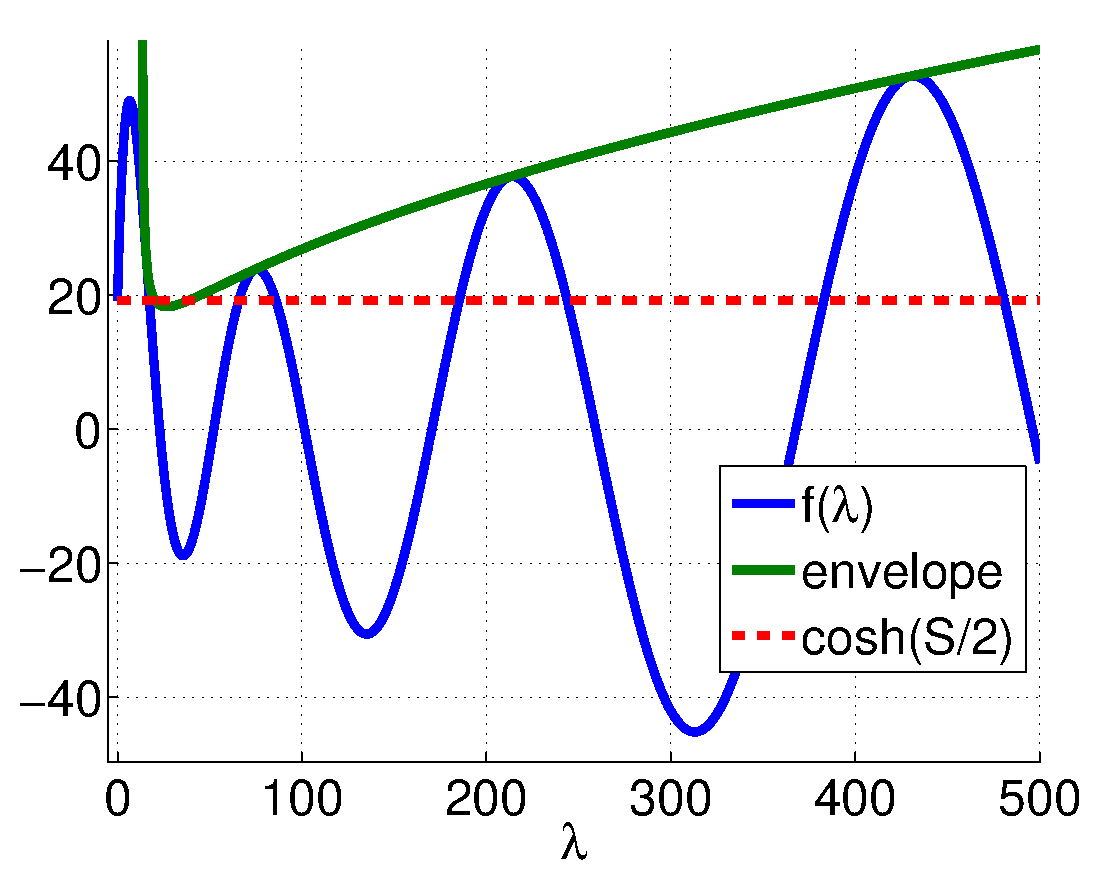
\includegraphics[height=4cm]{f_sg.eps}
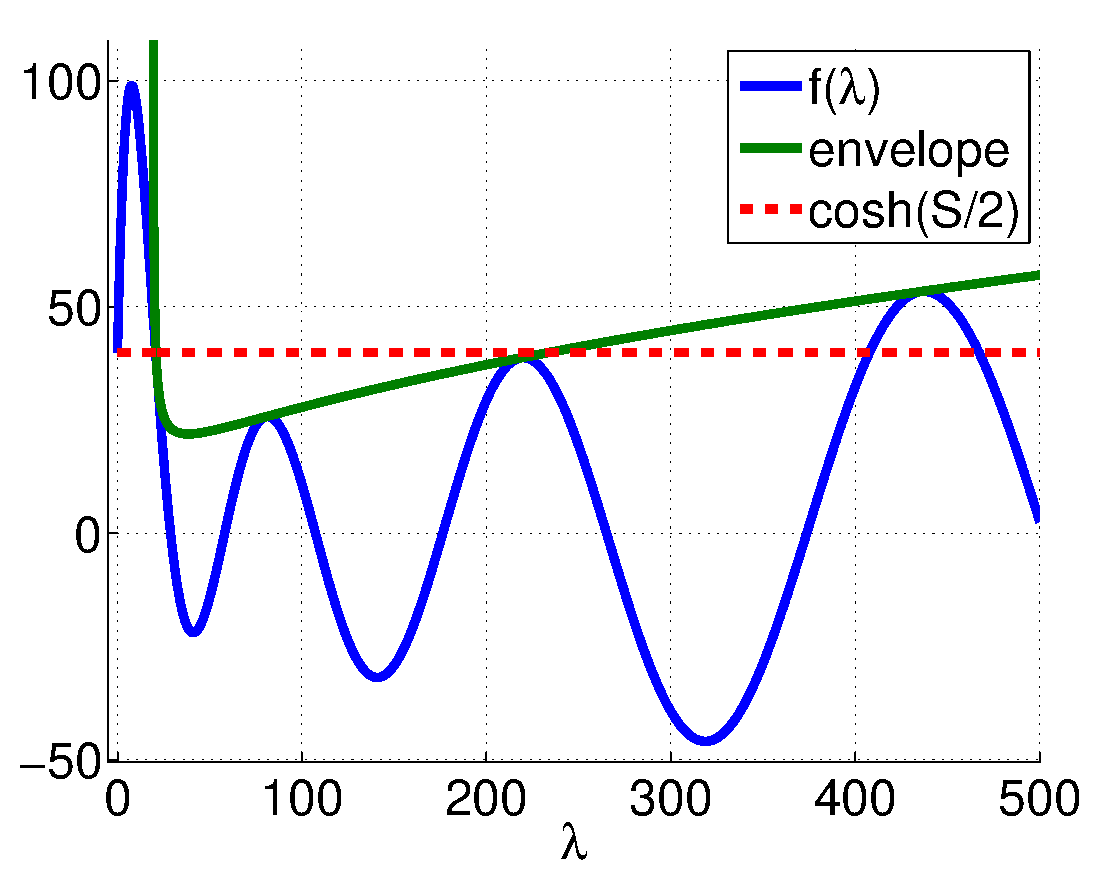
\includegraphics[height=4cm]{f_sg_p.eps}
\caption{The secular equation $f(\lambda)=\cosh(\mathcal{S}/2)$ for $g=5$ and $\mathcal{S} = 0.8 \mathcal{S}_g$ (left), $\mathcal{S} = \mathcal{S}_g$ (middle) and $\mathcal{S} = 1.2 \mathcal{S}_g$ (right).
In the right panel, the spectrum is initially real, then there is a complex eigenvalue and then the spectrum becomes real again. The high eigenvalues correspond to modes that decay very fast. Intuitively, since the high eigenvalues decay quickly, they cannot complete a trip around the ring before they decay, so they must be real.}
\label{fig_f}
\end{figure}
%%%%%%%%%%%%%%%%%%%%%%%%%%%%%%%%%%%


This is a transcendental equation with complex solutions $z=x+iy$. 
The solution $\lambda=0$, or $z=is/2$ is always a solution.
The remaining solutions can be found graphically and
from \Eq{e9} we can determine wether or not they are complex. 
A real solution $z=x$ is obtained at the intersection
of the oscillating l.h.s with the constant r.h.s..
The l.h.s is an oscillating function inside an envelope
%
\beq
\kappa = \sqrt{1+g^2 \left( \frac{x^2+(\frac{\mathcal{S}}{2})^2}{2x} \right)^2}
\eeq
%
Our goal is to explore the spectrum as a function of $\mathcal{S}$ and to determine 
wether the gap is complex or real.
%
For $\mathcal{S} \ll 1$, we expand \Eq{e9} near $x=0$

%
\beq
\lim_{x\to 0} \left[ \cos(x) + g \frac{x^2+(\frac{\mathcal{S}}{2})^2}{2x}\sin(x)\right] \ &=& \ 1+\frac{1}{2}g\left(\frac{\mathcal{S}}{2}\right)^2
\eeq
%
and small $\mathcal{S}$ on the r.h.s
%
\beq
\cosh\left(\frac{\mathcal{S}}{2}\right) & \approx & 1+\frac{1}{2}\left(\frac{\mathcal{S}}{2}\right)^2
\eeq
%
We see that there is a critical value $g_c=1$
such that for $g > g_c $, the envelope is above $\cosh(\mathcal{S}/2)$, so  the spectrum is real (\Fig{fig1}, left panel) and if  $g<g_c$ the envelope is beneath $\cosh(\mathcal{S}/2)$ and the spectrum is complex (\Fig{fig1}, right panel).

%%%%%%%%%%%%%%%%%%%%%%%%%%%%%%%%%%
\begin{figure}[h]
\includegraphics[height=5cm]{realGap.eps}
\includegraphics[height=5cm]{complexGap.eps}
\caption{Graphical representation of secular equation, assuming $z=x$ is real. The blue dashed curve is the envelope function and the black dashed line is $\cosh(\mathcal{S}/2)$.  For $g>g_c$ (left), all eigenvalues are real. For $g<g_c$ (right), the first eigenvalue is real, followed by complex eigenvalues and then real eigenvalues again. In these plots $s=1$, $g=2$ (left) and $g=0.1$ (right)}
\label{fig1}
\end{figure}

%%%%%%%%%%%%%%%%%%%%%%%%%%%%%%%%%%%

We would like to determine wether or not there is a gap between $\lambda=0$ and the 
rest of the spectrum. 
If the next eigenvalue is real, then the gap is "real", otherwise we say it is "complex". 
To do so, we must analyse \Eq{e9} more precisely. 
Restoring the imaginary component, such that $z=x+iy$, we write the eigenvalues
%
\beq
\lambda = (x+iy)^2+\left(\frac{\mathcal{S}}{2}\right)^2 = x^2-y^2 + \left(\frac{\mathcal{S}}{2}\right)^2 +2ixy
\eeq
%
For $g>g_c$ the solutions are real, as we have shown, and the eigenvalues are 
%
\beq
\lambda = x^2+ \left(\frac{\mathcal{S}}{2}\right)^2
\eeq
%
therefore there is always a gap due to $\mathcal{S}$. 
%

For $g<g_c$, 
%
We define 
%
\beq
Y(x) = \sqrt{x^2 + \left(\frac{\mathcal{S}}{2}\right)^2 }
\eeq
%
So the real part of $\lambda_1$ is 
%
\be{12}
\text{Re}[\lambda_1] = Y(x_1)^2-y_1^2
\ee
%
Since $\text{Re}[\lambda]>0$, the region $y>Y(x)$ is inaccessible, 
so to show that there is a gap it is enough to show that ${\text{Re}[\lambda_1]=Y(x_1)^2-y_1^2>0}$, where 
$\lambda_1$ is the eigenvalue with smallest and finite real part.
Assuming now that there is an imaginary part, such that $z= x+iy$,
\Eq{e9} becomes two equations for the real and imaginary parts. 
The real part equation \Eq{e9} is 
%
\be{10}
\cos (x) \left[ \cosh (y) - gy \sinh (y) \frac{x^2+y^2 - \mathcal{S}^2/4}{2(x^2+y^2)} \right]
+\sin(x) \left[ gx \cosh(y)\frac{x^2+y^2 + \mathcal{S}^2/4}{2(x^2+y^2)}   \right]
= \cosh\left(\frac{\mathcal{S}}{2}\right)
\ee
%
The imaginary part is 
%
\be{11}
\sin(x) \left[\sinh(y) - gy\cosh(y) \frac{x^2+y^2 - \mathcal{S}^2/4}{2(x^2+y^2)} \right]
-\cos(x) \left[gx \sinh(y)  \frac{x^2+y^2 + \mathcal{S}^2/4}{2(x^2+y^2)} \right] = 0
\ee
%
It is immediately seen that $\lambda(x=0,y=\mathcal{S}/2) = 0$ is a solution.
The remaining solutions can be found graphically.
%
In \Fig{fig2}, the real part (\Eq{e10}) is plotted for a several values of $y$. 
As $y$ increases, solutions appear, if $y$ is further increased, the solution bifurcates, the $y$ value at which this happens is the solution to the imaginary part (\Eq{e11}).
The first solution appears at $x_1\approx 2\pi(1+g/2)$, plugging this number in to the envelope of \Eq{e10} and demanding that the envelope and $\cosh(\mathcal{S}/2)$ intersect determines $y_1$.
%
In the limit $g\to 0$ we have a clean ring so all eigenvalues are complex with $y=is/2, x = 2\pi n$, for $g=g_c$ all eigenvalues are real and for $g>g_c$ they just spread out along the real axis in accordance with \Eq{e5}. 
%
\begin{figure}[h]
\includegraphics[height=5cm]{envelope_x.eps}
\includegraphics[height=5cm]{y_x_traj_gap.eps}
\caption{Left panel: Graphical representation of \Eq{e10} for $g=0.1, \ s=1$ and various $y$ values.
Right panel: the trajectories $y(x)$ computed from \Eq{e10}. The bifurcation points
are the complex solutions to \Eq{e9}. The solid black line is $Y(x)$, the region 
above the black line can not contain solutions. 
The  length of the dashed black line (the distance between the bifurcation point $y_1$ and the black line $Y(x_1)$ determines the gap according to \Eq{e12}.}
\label{fig2}
\end{figure}
%
\subsection{Model II - Ring with two drift regions}
In this section we analyse the simplest model to exhibit
the sliding transition.
In the region $0<x<L/2$ the drift velocity is $v_1$
and in the region $L/2<x<L$ the drift velocity is $v_2$.
In terms of $s$ and $\sigma$
%
\beq
v_1 &=& D(s+\sigma)\\
v_2 &=& D(s-\sigma)
\eeq
%

The secular equation for the eigenvalues can be shown to be 
%
\be{13}
\cosh\left(\frac{\mathcal{S}}{2}\right) &=&
%\cos\left[\frac{1}{2}\sqrt{z^2-\left(\frac{\sigma}{2}\right)^2 - \frac{\sigma s}{2}}\right]
%\cos\left[\frac{1}{2}\sqrt{z^2-\left(\frac{\sigma}{2}\right)^2 + \frac{\sigma s}{2}}\right]\\
%&-&\frac{z^2+\left(\frac{\sigma}{2}\right)^2}{\sqrt{\left(z^2-\left(\frac{\sigma}{2}\right)^2\right)^2-\left(\frac{\sigma s}{2}\right)^2}}
%\sin\left[\frac{1}{2}\sqrt{z^2-\left(\frac{\sigma}{2}\right)^2 - \frac{\sigma s}{2}}\right]
%\sin\left[\frac{1}{2}\sqrt{z^2-\left(\frac{\sigma}{2}\right)^2 + \frac{\sigma s}{2}}\right] = \\
%&=&
\cos\left[\frac{1}{2}\sqrt{z^2-\left(\frac{\sigma}{2}\right)^2 - \frac{\sigma \mathcal{S}}{2}}\right]
\cos\left[\frac{1}{2}\sqrt{z^2-\left(\frac{\sigma}{2}\right)^2 + \frac{\sigma \mathcal{S}}{2}}\right]-\\
&-&\left(z^2+\left(\frac{\sigma}{2}\right)^2\right)
\frac{\sin\left[\frac{1}{2}\sqrt{z^2-\left(\frac{\sigma}{2}\right)^2 - \frac{\sigma \mathcal{S}}{2}}\right]}{\sqrt{z^2-\left(\frac{\sigma}{2}\right)^2 - \frac{\sigma \mathcal{S}}{2}}}\
\frac{\sin\left[\frac{1}{2}\sqrt{z^2-\left(\frac{\sigma}{2}\right)^2 +\frac{\sigma \mathcal{S}}{2}}\right]}{\sqrt{z^2-\left(\frac{\sigma}{2}\right)^2 + \frac{\sigma \mathcal{S}}{2}}}  \nonumber
\ee
%
with additional solutions when
%
\be{14}
\left[z^2-\left(\frac{\sigma}{2}\right)^2 - \frac{\sigma \mathcal{S}}{2}\right]
\left[z^2-\left(\frac{\sigma}{2}\right)^2 + \frac{\sigma \mathcal{S}}{2} \right] =0
\ee
%
Note that the steady state solution $z_0=i\mathcal{S}/2$ is a solution to \Eq{e13}.
If we assume $z\geq 0$, then
%
\beq
z_{1,2} =  \sqrt{ \left(\frac{\sigma}{2}\right)^2 \pm \frac{\sigma \mathcal{S}}{2}   }
\eeq
%
The solution $z_1=\sqrt{(\sigma/2)^2 - \sigma s/2}$  corresponds to the smallest non zero real eigenvalue provided that $s<\sigma/2$ (see \Fig{realSpectrum}).
In this case, the gap is 
%
\be{15}
\text{Re}[\lambda_1]= z_1^2 + \frac{\mathcal{S}^2}{4} = \frac{1}{4}\left(\mathcal{S}-\sigma \right)^2
\ee
%
 If $s>\sigma/2$, $z_1$ is no longer a real solution, implying that the associated eigenvalue moved in to the complex plane. Thus, the critical value of $s$ for the gap to be complex is simply $s_c=\sigma/2$.
 For $\mathcal{S}>\mathcal{S}_c$, the gap is determined by \Eq{e13}. 
\rmrk{ For large enough $\mathcal{S}\gg \mathcal{S}_c$, 
 we should effectively have a clean ring, described by \Eq{e9} with $g=0$. However, I don't know how to show it from \Eq{e13}. The only limit I see, is that for ${z^2\gg (\sigma/2)^2 \pm \sigma s/2}$ we get 
 ${\cosh(\mathcal{S}/2)=\cos(z)}$.}

%%%%%%
\begin{figure}
\includegraphics[height=6.5cm]{realLambda_sigma_5}
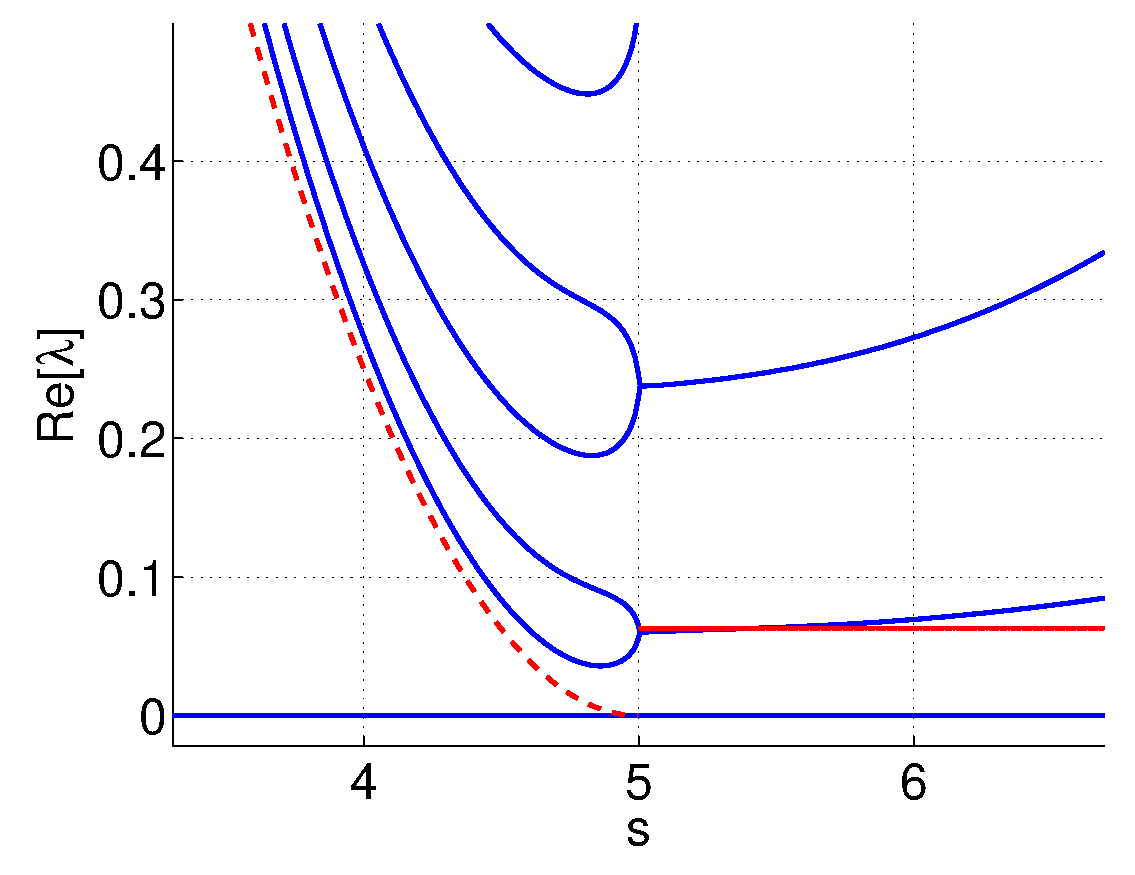
\includegraphics[height=6.5cm]{realLambda_sigma_5_N_50}
\caption{Left panel: The eigenvalues for an $N=10$ ring with two drift regions $\sigma=5$ plotted vs. the affinity $s$. Right panel: The same, but for $N=100$, focusing on the lower bands. The dashed red line corresponds to the solution $z_1$ of \Eq{e15}, the deviation is because of the tight binding approximation (finite size effect). The horizontal red line is $\text{Re}[\lambda] = 16\pi^2D/N^2$.}
\label{realSpectrum}
\end{figure}



\clearpage
%%%%%%%%%%%%%%%%%%%%%%%%%%%%%%%%%%%%%%%%%%%%%%%
\clearpage
%\section{Appendix - Diffusion equation with drift and varying diffusion coefficient}
%Consider the diffusion equation on a one dimensional ring $x\in [0,L]$
%%
%\be{1}
%\frac{\partial \psi}{\partial t} = \frac{\partial }{\partial x} \left[ D(x) \frac{\partial \psi}{\partial x}\right] - v\frac{\partial \psi}{\partial x}
%\ee
%%
%with diffusion coefficient 
%%
%\beq
%D(x) = \left\{ \begin{array}{cc}
%D_0, & |x|<a/2 \\
%D, & |x|>a/2 
%\end{array}
%\right.
%\eeq
%% 
%We will refer to this configuration as a "diffusion barrier".
%
%We ask the question - under what conditions is the reality of the spectrum broken. 
%Specifically we are interested in the limit $a\to 0$.
%%
%The solution to the diffusion equation in each region is  simply  $\psi \sim e^{-\lambda t + ikx}$, inserting this in \Eq{e1}, we obtain the dispersion relation 
%%
%\beq
%\lambda &=& Dk^2 + ivk\\
%k_{\pm} &=& \frac{-iv \pm \sqrt{4\lambda D -v^2}}{2D} = \frac{-is}{2} \pm \sqrt{\frac{\lambda}{D}-\frac{s^2}{4}}
%\eeq
%%
%So the solution to \Eq{e1} has the form 
%\be{2}
%\psi(x) = Ae^{ik_{+} x}+ Be^{ik_{-} x} = \eexp{\frac{v}{2D}x} \left(Ae^{i\frac{\sqrt{4\lambda D -v^2}}{2D}x}+Be^{-i\frac{\sqrt{4\lambda D -v^2}}{2D}x}\right)
%\ee

%%%%%%%%%%%%%%%%%%%%%%%%%%%%%%%%%%%%%%%%%%%%%%%%%%%%
%%%%%%%%%%%%%%%%%%%%%%%%%%%%%%%%%%%%%%%%%%%%%%%%%%%%
%
%\subsection{Simple cases}
%
%Let us first consider the simplest cases of a ring with and without drift and $D(x)=D$,
%We then compare to a chain (Neumann or Dirichlet boundary conditions)
%\begin{enumerate}
%\item
%$D(x)=D, \ v=0$ and periodic boundary conditions $\psi(0)=\psi(L), \ \psi'(0)=\psi'(L)$, we obtain the eigenvalues $-\lambda$
%%
%\be{3}
%\lambda  = Dk^2 =D\frac{4\pi^2 n^2}{L^2}
%\ee
%%
%So of course the spectrum is real. 
%%
%
%\item
% $D(x)=D, \ v/D=s \neq 0$ and periodic boundary conditions $\psi(0)=\psi(L), \ \psi'(0)=\psi'(L)$, we obtain the eigenvalues $-\lambda$
%%
%\be{4}
%\lambda &=&  D\frac{4\pi^2 n^2}{L^2}-i\omega n \\ 
%\omega &=& \frac{2\pi v}{L}
%\ee
%%
%The spectrum is complex except for $\lambda = 0$.
%\item  $D(x)=D, \ v/D=s \neq 0$  Neumann boundary conditions yield
%%
%\be{5}
%\lambda &=& D\frac{\pi^2 n^2}{L^2} + \frac{v^2}{4D}\\ 
%\lambda &=& 0
%\ee
%%
%Again, the spectrum is entirely real. 
%\end{enumerate}
%%%%%%%%%%%%%%%%%%%%%%%%%%%%%%%%%%%%%%%%%%%%%%%%%%%%
%%%%%%%%%%%%%%%%%%%%%%%%%%%%%%%%%%%%%%%%%%%%%%%%%%%%

\section{Appendix: Matching conditions across a "diffusion barrier"}
The diffusion barrier is defined as 
%
\beq
D(x) = \left\{ \begin{array}{cc}
D_0, & |x|<a/2 \\
D, & |x|>a/2 
\end{array}
\right.
\eeq
%
Requiring that the diffusion equation \Eq{e1} be continuous dictates that 
the distribution function $\psi(x)$ 
and the current $D(x)\partial_x \psi(x)-v\psi(x)$ 
be continuous.
This is in contrast to the Schroedenger equation, 
where the continuity requirement is on the derivative $\partial_x\psi(x)$ and not on the current. 
Let us denote the wave function inside the barrier $|x|<a/2$ as $\psi_0$. Outside, it is $\psi$.
%
\beq
\psi_0 &=& A e^{ik_0x} + Be^{-ik_0x} \\
\partial \psi_0 &=& ik_0\left(A e^{ik_0x} - Be^{-ik_0x}\right) \\
\eeq
%
where $k_0 = \sqrt{\lambda/D_0}$.
Since we will later take the limit $a\to 0$, we assume that the drift term doesn't play a role within the diffusion barrier. 

Inside the barrier, the probability distribution is freely propagating. The values of $\psi_0,\partial\psi_0$ at each of the boundaries $x=\pm a/2$ can be shown to be  related by the linear equation
%
\beq
\left.\left( \begin{array}{c}
\psi_0 \\
\partial \psi_0
\end{array}
\right)\right|_{-a/2} = 
\left( \begin{array}{cc}
\cos(k_0a) & \frac{1}{k_0} \sin{k_0a} \\
-k_0 \sin{k_0a} & \cos(k_0a)
\end{array}
\right)
\left.\left( \begin{array}{c}
\psi_0 \\
\partial \psi_0
\end{array}
\right)\right|_{a/2} 
\eeq
%

And requiring continuity of the distribution and the current, we can stitch the interior solution $\psi_0$ to the exterior solution $\psi$
%
\beq
\left.\left( \begin{array}{c}
\psi\\
\partial \psi
\end{array}
\right)\right|_{-a/2}  = 
%\left( \begin{array}{cc}
%1 & 0 \\
%0 & \frac{D_0}{D}
%\end{array}
%\right)
%\left( \begin{array}{cc}
%\cos(k_0a) & \frac{1}{k_0} \sin{k_0a} \\
%k_0 \sin{k_0a} & \cos(k_0a)
%\end{array}
%\right)
%\left( \begin{array}{cc}
%1 & 0 \\
%0 & \frac{D}{D_0}
%\end{array}
%\right)
%\left.\left( \begin{array}{c}
%\psi \\
%\partial \psi
%\end{array}
%\right)\right|_{a/2} = \\
\left( \begin{array}{cc}
\cos(k_0a) & \frac{D}{D_0 k_0} \sin{k_0a} \\
-\frac{D_0 k_0}{D} \sin{k_0a} & \cos(k_0a)
\end{array}
\right)
\left.\left( \begin{array}{c}
\psi \\
\partial \psi
\end{array}
\right)\right|_{a/2}
\eeq
%
Taking, carefully, the limit $a\to 0$, 
%
\beq
\left.\left( \begin{array}{c}
\psi\\
\partial \psi
\end{array}
\right)\right|_{-a/2}  \approx
\left( \begin{array}{cc}
1 & D\frac{a}{D_0 }  \\
0 & 1
\end{array}
\right)
\left.\left( \begin{array}{c}
\psi \\
\partial \psi
\end{array}
\right)\right|_{a/2}
\eeq
%
rewriting these two equations explicitly, we obtain the diffusion barrier matching conditions
%
\be{6}
\psi(a/2)-\psi(-a/2) &=& -\frac{a}{D_0}D \partial \psi(a/2)\\
\partial \psi(a/2) &=& \partial \psi(-a/2) 
\ee
%
To check, notice that if $D_0 \to 0$ faster than $a\to 0$, Neumann boundary conditions are recovered.\\
If $D_0=D$, periodic boundary conditions are recovered. 
Let us define 
%
\beq
\alpha \ = \ \frac{a}{D_0}\
\eeq
%
as the strength of the diffusion barrier, in analogy with a delta function potential in the schroedenger equation $u\delta(x)$.
%%%%%%%%%%%%%%%%%%%%%%%%%%%%%%%%%%%%%%%%%%%%%%%%%%%%
%%%%%%%%%%%%%%%%%%%%%%%%%%%%%%%%%%%%%%%%%%%%%%%%%%%%
\subsection{Eigenvalues of the diffusion barrier problem}
Using the boundary conditions of \Eq{e6} and the solution of the form of \Eq{e2}, 
the following equation for the eigenvalues is obtained
%
\be{7}
\cos(\tilde{k}L) + \alpha \frac{\lambda}{2\tilde{k}}\sin(\tilde{k}L) = \cosh(sL/2)
\ee
%
which can also be written simply as 
%
\beq
\sqrt{1+\alpha^2\frac{\lambda^2}{4\tilde{k}^2}} \cos \left[ \tilde{k}L - \arctan \left(\alpha\frac{ \lambda}{2\tilde{k}}\right)\right] = \cosh(sL/2)
\eeq
%
where  
\beq
\tilde{k} &\equiv & k + \frac{is}{2} =  \sqrt{\frac{\lambda}{D}-\frac{s^2}{4}} 
\eeq
%

%

In more conventional notations, \Eq{e7} can be written as follows
%
\be{8}
\cos\left( \gamma(\lambda)\right) = \sqrt{g(\lambda)} \cosh\left(\frac{sL}{2}\right)
\ee
%
where
%
\beq
g(\lambda) = \left[1+\left(\frac{\lambda}{2\tilde{k}}\alpha\right)^2\right]^{-1}
\eeq
%
and 
%
\beq
\gamma(\lambda) =  \tilde{k}L - \arctan \left(\frac{ \lambda}{2\tilde{k}}\alpha\right) 
\eeq
%
We immediately conclude that for $s=0$ all eigenvalues are real. \\
For $s\neq0$ and $\alpha=0$ all eigenvalues (except for $\lambda=0$) are complex. This corresponds to a fully connected ring.
As $\alpha$ increases the ring becomes disconnected and more and more eigenvalues become real. 
%
For given $\alpha$, as $s$ increases the eigenvalues become complex. The indication for this 
is that the real part of the eigenvalues coalesce and the imaginary part bifurcates (See \Fig{discrete}, for a discrete ring).


By inspection of \Eq{e8} it is evident that 
when the right hand side of the equation is greater than one,
the argument $\gamma(\lambda)$ must be complex.
%
This is the case when $\mbox{Re}[\lambda(s)] < \lambda^*(s)$ (see \Fig{lambda_star}):
%
\be{19}
\lambda^* (s) \ = \ \frac{2}{\alpha^2 D} \sinh^2\left(\frac{sL}{2}\right) \left[1+ \sqrt{1 - \left(\frac{\alpha Ds}{2\sinh\left(\frac{sL}{2}\right)}\right)^2} \right]
\ee


\begin{figure}[h]
\includegraphics[height=6.5cm]{lambda_star.eps}
\caption{The real part of the eigenvalues for an $L=35, \ D=1$ ring with a single diffusion barrier with $\alpha=10$ plotted vs. the affinity $s$.
The black line is the $\mbox{Re}[\lambda^{*}(s)]$ of \Eq{e9}, which indicates where the eigenvalues become complex. 
The dashed blue lines are the eigenvalues of the disconnected ring with $s=0$, \Eq{e5}.
Given a high frequency cutoff $\lambda_c$, we can invert \Eq{e19} to obtain $s_c = s(\lambda_c)$, if $s>s_c$, all eigenvalues within the region $\lambda<\lambda_c$ are complex.
}
\label{lambda_star}
\end{figure}
\begin{figure}
\includegraphics[height=6.5cm]{ReLambda_s_1.eps}
\includegraphics[height=6.5cm]{ImLambda_s_1.eps}
\caption{The eigenvalues for an $N=25$ ring with a single diffusion barrier with $g=\exp(-7.5)$ plotted vs. the affinity $s$.}
\label{discrete}
\end{figure}



%\subsection{Eigenvalues of tight binding model with disorder}
%The following results are for $N=35$ sites and $500$ realizations.
%The connectivity of each bond is a random number from a log-box distribution with log width $\Delta$.
%\begin{figure}
%\includegraphics[height=6.5cm]{/Figs/meanNumReal.eps}
%\includegraphics[height=6.5cm]{/Figs/stdNumReal.eps}
%\includegraphics[height=6.5cm]{/Figs/NumReal.eps}
%\caption{Top row from left to right: Mean number of real eigenvalues, standard deviation of number of eigenvalues. 
%Bottom: number of real eigenvalues of a single realization. The horizontal axis is the affinity per unit length and the vertical axis is the weakest link. }
%\end{figure}
%
%\begin{figure}
%\includegraphics[height=6.5cm]{/Figs/ReLambda_s.eps}
%\includegraphics[height=6.5cm]{/Figs/ImLambda_s.eps}
%\caption{The eigenvalues for an $N=15$ ring with disorder, $\Delta = 0.5$ plotted vs. the affinity $s$.}
%\end{figure}
%

%%%%%%%%%%%%%%%%%%%%%%%%%%%%%%%%%%%

\section{Appendix - Ring with two drift regions: Details of derivation}
Details of the derivation  of \Eq{e13} and \Eq{e14} are as follows:
The diffusion equation with space dependent drift is 
%
\be{15}
\frac{\partial \psi}{\partial t} = D \frac{\partial^2 \psi}{\partial x^2}- \frac{\partial}{\partial x} \left[v(x)\psi\right]
\ee
%
with 
%
\beq
v(x) = \left\{ \begin{array}{cc}
v_1, & 0< x<L/2 \\
v_2, & L/2<x<L
\end{array}
\right.
\eeq
%
and
% 
\beq
v_1 &=& s_1 D = D(s+\sigma)\\
v_2 &=& s_2 D = D(s-\sigma)
\eeq
%
The solutions are of the form $\psi \sim e^{-\lambda t + ikx}$. In each region $(1,2)$ we have two $k$'s, $\pm$:
\beq
k_{1,2}^{\pm} = \frac{-iv_{1,2} \pm \sqrt{4\lambda D - v_{1,2}^2}}{2D} = -\frac{is_{1,2}}{2} \pm \sqrt{\frac{\lambda}{D}-\frac{s_{1,2}^2}{4}} \equiv  -\frac{is_{1,2}}{2} \pm k_{1,2}
\eeq
%
In each region we may write the solution, i.e.:
%
\beq
\psi_1(x) &=& A e^{ik_1^+ x} + B e^{ik_1^- x} \\
\partial_x \psi_1(x) &=& ik_1^+ A e^{ik_1^+ x} + ik_1^- B e^{ik_1^- x} 
\eeq
%
From which we can obtain the connection between $(\psi,\partial \psi)$ at any two points, specifically for the boundaries of the region $[0,L/2]$ we have
%
\beq
\left.\left( \begin{array}{c}
\psi_1 \\
\partial \psi_1
\end{array}
\right)\right|_{x=0} = 
%
T(s_1,k_1)
%
\left.\left( \begin{array}{c}
\psi_1 \\
\partial \psi_1
\end{array}
\right)\right|_{x=L/2} 
\eeq
%
where 
%
\beq
T(s,k;L/2)\equiv
\frac{e^{s L/4}}{k}
\left(
\begin{array}{cc}
-\frac{s}{2}\sin\left(\frac{k L}{2}\right) + k\cos \left(\frac{k L}{2}\right) & \sin\left(\frac{k L}{2}\right)\\
-\left(\frac{s^2}{4}+k^2\right)\sin \left(\frac{k L}{2}\right) & \frac{s}{2} \sin \left(\frac{k L}{2}\right) + k \cos \left(\frac{k L}{2}\right)
\end{array}
\right)
\eeq
Continuity of the diffusion equation across the boundaries requires that 
the distribution $\psi$ and the current $D\partial \psi -v \psi$ be contiuous across the boundaries
%
\beq
\left.\left( \begin{array}{c}
\psi_1 \\
\partial \psi_1
\end{array}
\right)\right|_{x=L/2} = 
%
M(v_1-v_2)
%
\left.\left( \begin{array}{c}
\psi_2 \\
\partial \psi_2
\end{array}
\right)\right|_{x=L/2}
\eeq
%
where
%
\beq
M(u) \equiv
\left( \begin{array}{cc}
1 &0  \\
\frac{u}{D} & 1
\end{array}
\right)
\eeq
%
To find $\lambda$, we apply these transformations along the entire segment $[0,L]$ and impose periodic boundary conditions
%
\beq
\left.\left( \begin{array}{c}
\psi_1 \\
\partial \psi_1
\end{array}
\right)\right|_{x=0}  = 
T(s_1,k_1) M(v_1-v_2) T(s_2,k_2) M(v_2-v_1)
\left.\left( \begin{array}{c}
\psi_1 \\
\partial \psi_1
\end{array}
\right)\right|_{x=0} 
\eeq
%
This equation has a non trivial solution only if 
%
\beq
\det \left[ I - T(s_1,k_1) M(v_1-v_2) T(s_2,k_2) M(v_2-v_1) \right] = 0
\eeq
%
We Define $k$ as in the $\sigma=0$ case, such that
%
\beq
\lambda \ = \ D\left( {k}^2 + \frac{s^2}{4}\right) \ = \ \frac{D}{L^2}\left( {z}^2 + \frac{\mathcal{S}^2}{4}\right) 
\eeq
%
%
\beq
z \  \equiv  {k}L \ \ , \ \ \mathcal{S} \equiv sL
\eeq
%
where $z=x+iy$ is complex,
and calculate the determinant to obtain  the equation
%
\beq
& & 
\left[4z^2-\sigma(2s+\sigma)\right]
\left[4z^2 +\sigma(2s - \sigma) \right]
\cosh\left(\frac{s}{2}\right) = \\
&=&
\left[4z^2-\sigma(2s+\sigma)\right]
\left[4z^2 +\sigma(2s - \sigma) \right]
\cos \left(\frac{1}{4} \sqrt{4z^2-\sigma(2s+\sigma)}\right) 
\cos \left(\frac{1}{4} \sqrt{4z^2 +\sigma(2s - \sigma)}\right)  -\\
&-& 
(4z^2+\sigma^2) \sqrt{4z^2-\sigma(2s+\sigma)}
\sqrt{4z^2 +\sigma(2s - \sigma)}
\sin \left(\frac{1}{4} \sqrt{4z^2-\sigma(2s+\sigma)}\right) 
\sin \left(\frac{1}{4} \sqrt{4z^2 +\sigma(2s - \sigma)}\right)  
\eeq
%
%The first real solution for $\lambda$ is $\lambda=0$, which means $z=i\mathcal{S}/2$.
%We would like to determine wether the next eigenvalue is real or complex. 
%The next real solution is obtained when the above equation has a real $z$ solution.



\end{document}
%%%%%%%%%%%%%%%%%%%%%%%%%%%%%%%%%%%%%%%%%%%%%%%%%%%%%%%%%%%%%%%%%%
